\documentclass{article}

\usepackage[top=3cm, bottom=3cm, left=3cm,right=3cm]{geometry}
\usepackage[colorinlistoftodos]{todonotes}
\usepackage{graphicx}
\usepackage{amssymb}
\usepackage{amsmath}
\usepackage{bbm}
\usepackage{todonotes}
\usepackage{pdflscape}
\usepackage{caption}
\usepackage{subcaption}
\usepackage[T1]{fontenc}
\usepackage[utf8]{inputenc}
\usepackage{authblk}
\usepackage{pdfpages}
\usepackage{setspace} 
\usepackage{booktabs}
\usepackage{longtable}
\usepackage{float}
\usepackage{tikz}
\usepackage[colorlinks=true,citecolor=blue, linkcolor=blue]{hyperref}
\usepackage{multirow}
\usepackage{todonotes}
\setlength{\tabcolsep}{5pt}
%%\setlength{\parindent}{0pt}
\usepackage[parfill]{parskip}
\renewcommand{\arraystretch}{1.5}

\renewcommand\Affilfont{\itshape\footnotesize}
\def\ci{\perp\!\!\!\perp}

\renewcommand\Affilfont{\itshape\footnotesize}
\linespread{1.5}

% \usepackage{lineno}
% \linenumbers

% Nature Bibliography style
\usepackage[backend=biber,style=nature]{biblatex}
\addbibresource{library.bib} 

%%%%%%%%%%%%%
%%% Title %%%
%%%%%%%%%%%%%
\title{District-level male medical and traditional circumcision coverage and unmet need in sub-Saharan Africa}

\author{}
\date{}

%%%%%%%%%%%%%%%%%%%%%%%%%%%%%%%%%%%%%%%%%%%%%%%%%%%%%%%%%%%%%%%%%%
%%%%%%%%%%%%%%%%%%%%%%%%%%%%%%%%%%%%%%%%%%%%%%%%%%%%%%%%%%%%%%%%%%
%%%%%%%%%%%%%%%%%%%%%%%%%%%%%%%%%%%%%%%%%%%%%%%%%%%%%%%%%%%%%%%%%%

\begin{document}

%%%%%%%%%%%%%%%%%%%%%%%%%%%%%%%%%%%%%%%%%%%%%%%%%%%%%%%%%%%%%%%%%%
%%%%%%%%%%%%%%%%%%%%%%%%%%%%%%%%%%%%%%%%%%%%%%%%%%%%%%%%%%%%%%%%%%
%%%%%%%%%%%%%%%%%%%%%%%%%%%%%%%%%%%%%%%%%%%%%%%%%%%%%%%%%%%%%%%%%%

\maketitle

\vspace{-1cm}

Patrick O'Toole\textsuperscript{1,2},
Matthew L. Thomas\textsuperscript{1,3,4},
Oliver Stevens\textsuperscript{1},
Kevin Lam\textsuperscript{1,5},
Katharine Kripke\textsuperscript{6},
Rachel Esra\textsuperscript{1},
Ian Wanyeki\textsuperscript{7},
Lycias Zembe\textsuperscript{7},
Jeffrey W. Imai-Eaton\textsuperscript{1,8} \\
\smallskip

\textbf{1} MRC Centre for Global Infectious Disease Analysis, School of Public Health, Imperial College London, London, United Kingdom\\
\textbf{2} Department of Mathematical Sciences, University of Bath, Bath, United Kingdom\\
\textbf{3} Department of Earth and Environmental Sciences, University of Manchester, Manchester, United Kingdom\\
\textbf{4} National Centre for Atmospheric Sciences, University of Manchester, Manchester, United Kingdom\\
\textbf{5} Department of Statistics, University of British Columbia, Vancouver, Canada\\
\textbf{6} Avenir Health, Washington, District of Columbia, United States of America\\
\textbf{7} Joint United Nations Programme on HIV/AIDS (UNAIDS), Geneva, Switzerland\\
\textbf{8} Center for Communicable Disease Dynamics, Department of Epidemiology, Harvard T.H. Chan School of Public Health, Boston, Massachusetts, United States of America\\

\smallskip

* Corresponding Author Email

\clearpage


%%%%%%%%%%%%%%%%%%%%%%%%%%%%%%%%%%%%%%%%%%%%%%%%%%%%%%%%%%%%%%%%%%
%%%%%%%%%%%%%%%%%%%%%%%%%%%%%%%%%%%%%%%%%%%%%%%%%%%%%%%%%%%%%%%%%%
%%%%%%%%%%%%%%%%%%%%%%%%%%%%%%%%%%%%%%%%%%%%%%%%%%%%%%%%%%%%%%%%%%

\begin{abstract}
  \noindent \textbf{Background} \\

  \noindent \textbf{Methods} \\

  \noindent \textbf{Results} \\

  \noindent \textbf{Conclusions} \\

\end{abstract}
\newpage

%%%%%%%%%%%%%%%%%%%%%%%%%%%%%%%%%%%%%%%%%%%%%%%%%%%%%%%%%%%%%%%%%%
%%%%%%%%%%%%%%%%%%%%%%%%%%%%%%%%%%%%%%%%%%%%%%%%%%%%%%%%%%%%%%%%%%
%%%%%%%%%%%%%%%%%%%%%%%%%%%%%%%%%%%%%%%%%%%%%%%%%%%%%%%%%%%%%%%%%%

\section*{Introduction}

%%%%%%%%%%%%%%%%%%%%%%%%%%%%%%%%%%%%%%%%%%%%%%%%%%%%%%%%%%%%%%%%%%
%%%%%%%%%%%%%%%%%%%%%%%%%%%%%%%%%%%%%%%%%%%%%%%%%%%%%%%%%%%%%%%%%%
%%%%%%%%%%%%%%%%%%%%%%%%%%%%%%%%%%%%%%%%%%%%%%%%%%%%%%%%%%%%%%%%%%

The HIV epidemic remains a major public health challenge, despite substantial progress over the past two decades. In sub-Saharan Africa, the Joint United Nations Programme on HIV/AIDS (UNAIDS) estimates that over 26 million people were living with HIV in 2024, and around 650,000 people newly acquired HIV, accounting for half of all new HIV infections globally \cite{UNAIDS2025}. To achieve the global goal of ending AIDS as a public health threat by 2030, further progress in HIV prevention is required \cite{UNAIDSStrategy}. Voluntary medical male circumcision (VMMC) is a safe, effective and cost-effective one-time intervention to reduce HIV incidence \cite{bansi2023cost}, reducing female-to-male acquisition of HIV by approximately 60\% \cite{gray2007male, bailey2007male, auvert2005randomized, gray2012effectiveness}. Furthermore, evidence suggests VMMC may decrease the risk of HIV acquisition among men who have sex with men \cite{yuan2019circumcision}, and reduce the risk of other sexually transmitted infections \cite{tobian2009male, grund2017association}. 

\noindent In 2007, the World Health Organization (WHO) and UNAIDS recommended male circumcision as an additional HIV prevention intervention in settings with high heterosexual HIV prevalence and low male circumcision coverage \cite{WHOUNAIDS2007MC}. This led to the large-scale expansion of VMMC programmes across what ultimately became fifteen priority countries in eastern and southern Africa: Botswana, Eswatini, Ethiopia, Kenya, Lesotho, Malawi, Mozambique, Namibia, Rwanda, South Africa, South Sudan, Tanzania, Uganda, Zambia, and Zimbabwe \cite{UNAIDSJoint, davis2018progress, WHOVoluntary2}. Successive global strategies established ambitious coverage targets, initially aiming for at least 80\% circumcision coverage among men aged 15--49 years and subsequently 90\% coverage among adolescent boys and young men aged 10--29 years \cite{WHOJointFramework, WHOFramework}. Between 2008 and 2023, approximately 37.5 million VMMCs were conducted  across the 15 priority countries, supported by national governments and international programmes including the US President's Emergency Plan for AIDS Relief (PEPFAR) \cite{UNAIDS2025}. This has substantially altered the landscape of circumcision coverage across the region, with male circumcision coverage across eastern and southern Africa increasing from approximately 40\% to 56\% between 2010 and 2023 \cite{UNAIDS2025}. However, circumcision coverage remains highly heterogeneous between countries and substantially below previous targets in much of southern Africa.

\noindent In 2025, the policy and financing environment supporting VMMC scale-up changed markedly following abrupt reductions in United States funding, with VMMC activities reduced or paused in several PEPFAR-supported countries \cite{UNAIDS2025}. Against this backdrop, the UNAIDS Global AIDS Strategy 2026--2031 recommends that countries reassess the role of VMMC according to their epidemiological context and, where it remains cost-effective, integrate it into domestically financed health service provision \cite{UNAIDSStrategy}. Understanding the future role of male circumcision in HIV prevention therefore requires detailed estimates of overall circumcision coverage and how it varies by age, region, and circumcision type. Such estimates are needed to (i) characterise how the circumcision landscape has changed, (ii) inform the future planning and delivery of VMMC services, particularly as programmes transition towards more sustainable models of provision, and (iii) support evaluation of the impact of VMMC campaigns on HIV incidence. 

\noindent Although the large-scale provision of medical male circumcision (MMC) for HIV prevention is a relatively recent phenomenon, male circumcision has long been practised for traditional, cultural and religious reasons across much of sub-Saharan Africa \cite{WHOGlobalMC, lawal2017circumcision}. Traditional male circumcision (TMC), commonly undertaken as part of male initiation ceremonies, varies considerably between and within countries in its prevalence and the age at which circumcision occurs \cite{wilcken2010traditional}. For example, there is substantial geographical variation in traditional circumcision practices in South Africa, with traditional circumcision coverage among men aged 15–49 years ranging from around 5\% in KwaZulu-Natal to almost 50\% in Eastern Cape, and the average age at traditional circumcision varying from approximately 12 years in Limpopo to around 20 years in Western Cape \cite{thomas2024substantial}. TMC is often performed in non-clinical settings by traditional practitioners with no formal medical training and, in some populations, may not involve complete removal of the foreskin \cite{wilcken2010traditional, WHOTraditional, bailey2008male}. As a result, evidence that TMC provides the full HIV prevention benefits as complete medical circumcision is mixed \cite{shaffer2007protective, maffioli2017traditional, asa2023traditional}. In some settings, medical circumcision has also been integrated with traditional initiation practices, with initiates receiving VMMC before traditional rites or medical providers performing circumcisions within traditional male initiation ceremonies \cite{bulled2016making, thomas2024substantial}. Total male circumcision coverage can therefore reflect very different combinations of longstanding traditional practices and more recent medical intervention, with different implications for HIV prevention.

\noindent Many of the existing methods of estimating male circumcision coverage do not fully characterise these dynamics. Cork {\it et al.} \cite{cork2020mapping} developed a Bayesian geostatistical model using household survey data to estimate annual circumcision coverage among men aged 15–49 years across 38 countries in sub-Saharan Africa between 2000 and 2017. The analysis demonstrated substantial geographical heterogeneity in male circumcision coverage, including large differences within VMMC priority countries, but they combined medical and traditional circumcision and did not explicitly represent how circumcision accumulated by age within successive birth cohorts. Kripke {\it et al.} \cite{kripke2016age, kripke2016cost} developed the Decision Makers’ Program Planning Toolkit, Version 2 (DMPPT2), a compartmental model that combined survey-derived estimates of circumcision coverage with reported VMMC programme volumes to estimate coverage and unmet need by age and geography. Earlier implementations did not formally incorporate more recent household survey observations or quantify statistical uncertainty associated with coverage estimates. 

\noindent More recently, Thomas {\it et al.} \cite{thomas2024substantial} developed a Bayesian competing-risks time-to-event model that estimated medical and traditional circumcision by single-year age, district and time while synthesising household survey and VMMC programme data in South Africa. The analysis demonstrated that increases in total circumcision coverage concealed distinct changes in medical and traditional circumcision and substantial geographical variation in both practices. However, incorporating programme data required detailed knowledge of country-specific VMMC implementation, including the provision of medical circumcision within traditional initiation ceremonies and migration for circumcision, limiting straightforward application of the approach across multiple countries. 

\noindent In this paper, we extend the competing-risks time-to-event framework from Thomas {\it et al.} \cite{thomas2024substantial} to characterise the changing landscape of male circumcision across sub-Saharan Africa using nationally representative household survey data. We estimate annual probabilities and coverage of medical and traditional male circumcision by subnational area, single-year age and time, along with measures of uncertainty, for 34 countries between 2008 and 2023. We use these estimates to quantify geographical and demographic variation in medical and traditional circumcision practices, assess how the expansion of medical circumcision has changed circumcision coverage across successive cohorts, and identify populations in which low overall or medical circumcision coverage may represent remaining gaps in HIV prevention. 

%This analysis provides a comprehensive picture of the male circumcision landscape produced during the period of large-scale VMMC expansion and establishes a baseline immediately preceding recent major changes to international HIV prevention, against which the sustainability of these gains and the future role of VMMC across sub-Saharan Africa can be assessed. Move to discussion. 

%%%%%%%%%%%%%%%%%%%%%%%%%%%%%%%%%%%%%%%%%%%%%%%%%%%%%%%%%%%%%%%%%%
%%%%%%%%%%%%%%%%%%%%%%%%%%%%%%%%%%%%%%%%%%%%%%%%%%%%%%%%%%%%%%%%%%
%%%%%%%%%%%%%%%%%%%%%%%%%%%%%%%%%%%%%%%%%%%%%%%%%%%%%%%%%%%%%%%%%%

\section*{Methods}

%%%%%%%%%%%%%%%%%%%%%%%%%%%%%%%%%%%%%%%%%%%%%%%%%%%%%%%%%%%%%%%%%%
%%%%%%%%%%%%%%%%%%%%%%%%%%%%%%%%%%%%%%%%%%%%%%%%%%%%%%%%%%%%%%%%%%
%%%%%%%%%%%%%%%%%%%%%%%%%%%%%%%%%%%%%%%%%%%%%%%%%%%%%%%%%%%%%%%%%%

\subsection*{Data}

%%%%%%%%%%%%%%%%%%%%%%%%%%%%%%%%%%%%%%%%%%%%%%%%%%%%%%%%%%%%%%%%%%
%%%%%%%%%%%%%%%%%%%%%%%%%%%%%%%%%%%%%%%%%%%%%%%%%%%%%%%%%%%%%%%%%%

\subsubsection*{Study Region}

%%%%%%%%%%%%%%%%%%%%%%%%%%%%%%%%%%%%%%%%%%%%%%%%%%%%%%%%%%%%%%%%%%

We included 34 countries across sub-Saharan Africa with household surveys conducted since 2002 that collected information on self-reported circumcision status in this study. For modelling purposes, countries were classified into three groups according to VMMC priority status and the availability of information on circumcision type. The first group comprised 14 VMMC priority countries: Botswana, Eswatini, Ethiopia, Kenya, Lesotho, Malawi, Mozambique, Namibia, Rwanda, South Africa, Tanzania, Uganda, Zambia, and Zimbabwe. The second group comprised 15 non-priority countries: Angola, Benin, Burkina Faso, Burundi, Cameroon, Chad, Côte d’Ivoire, Gabon, Gambia, Ghana, Mali, Nigeria, the Republic of the Congo (the Congo), Sierra Leone, and Togo. The third group had survey information on circumcision status but insufficient information on circumcision type and were therefore analysed using a simplified model: the Democratic Republic of the Congo (DR Congo), Guinea, Liberia, Niger, and Senegal. Central African Republic, Equatorial Guinea, Guinea-Bissau, and South Sudan were excluded because no eligible surveys were available, or available surveys did not collect sufficient information on circumcision status for inclusion in the analysis (see below).

%%%%%%%%%%%%%%%%%%%%%%%%%%%%%%%%%%%%%%%%%%%%%%%%%%%%%%%%%%%%%%%%%%

\subsubsection*{Household surveys}

%%%%%%%%%%%%%%%%%%%%%%%%%%%%%%%%%%%%%%%%%%%%%%%%%%%%%%%%%%%%%%%%%%

In total, we identified 120 nationally representative household surveys conducted across sub-Saharan Africa between 2002 and 2023 that collected information on self-reported circumcision status. These comprised several major survey series, including the Demographic and Health Surveys (DHS) \cite{dhs}, AIDS Indicator Surveys (AIS) \cite{ais}, Population-based HIV Impact Assessment (PHIA) surveys \cite{phia}, Multiple Indicator Cluster Surveys (MICS) \cite{mics}, and, in South Africa, Human Sciences Research Council (HSRC) surveys \cite{hsrc}. We excluded five surveys because they did not collect the information on age at circumcision required for modelling: the 2008 and 2013 Botswana AIDS Impact Surveys (BAIS), the 2018 Central African Republic MICS, and the 2014 and 2018 Guinea-Bissau MICS. Supplementary Figure S1 summarises the surveys available for each country by survey provider, together with their sample sizes and the availability of information on circumcision type.

From each survey, we extracted age at the time of survey, survey cluster, and sampling weight for all male respondents, together with the following circumcision-related information where available: (i) self-reported circumcision status; (ii) age at circumcision; (iii) who performed the circumcision (health worker/professional, traditional practitioner, other, or unknown); and (iv) where the circumcision took place (health facility, home of a health worker/professional, respondent's home, ritual site, other, or unknown). To assign respondents geographically, we matched survey clusters to their accompanying (masked) geographic coordinates and used these to identify the corresponding primary sub-national unit (PSNU; hereafter referred to as the district). Geographic coordinates were unavailable for some surveys; in these cases, respondents were assigned to the finest geographic unit identified in the survey data, most commonly first-level administrative units. Survey respondents were excluded if they were missing any required demographic information or had missing circumcision status. Supplementary Table 1 summarises the circumcision-related variables available in each survey and the corresponding analytical sample sizes. We classified circumcision as medical male circumcision (MMC), traditional male circumcision (TMC), or male circumcision of unknown type (unknown MC) based jointly on responses to the questions ‘Who performed the circumcision?’ and ‘Where did the circumcision take place?’, according to the classification criteria described in Supplementary Table 2.

%%%%%%%%%%%%%%%%%%%%%%%%%%%%%%%%%%%%%%%%%%%%%%%%%%%%%%%%%%%%%%%%%%

\subsubsection*{Administrative boundaries }

%%%%%%%%%%%%%%%%%%%%%%%%%%%%%%%%%%%%%%%%%%%%%%%%%%%%%%%%%%%%%%%%%%

We obtained district boundaries and their nesting within higher administrative levels from the Combined Geographic Health Boundaries available through the UNAIDS AIDS Data Repository \cite{UNAIDSADR}.

%%%%%%%%%%%%%%%%%%%%%%%%%%%%%%%%%%%%%%%%%%%%%%%%%%%%%%%%%%%%%%%%%%

\subsubsection*{Population data}

%%%%%%%%%%%%%%%%%%%%%%%%%%%%%%%%%%%%%%%%%%%%%%%%%%%%%%%%%%%%%%%%%%

We obtained estimates of the male population by 5-year age group from 2008 to 2023 from WorldPop \cite{worldpop}. Unconstrained country-level male population rasters at 100 m spatial resolution were overlaid with the UNAIDS administrative boundaries and aggregated to the corresponding administrative units \cite{UNAIDSADR}. Population estimates were then scaled to align with national population totals from the United Nations Population Division World Population Prospects 2019 \cite{wpp}. Finally, population estimates by 5-year age group were disaggregated to single-year ages using Beers' ordinary interpolation formula \cite{beersmethod, beers}.

%%%%%%%%%%%%%%%%%%%%%%%%%%%%%%%%%%%%%%%%%%%%%%%%%%%%%%%%%%%%%%%%%%
%%%%%%%%%%%%%%%%%%%%%%%%%%%%%%%%%%%%%%%%%%%%%%%%%%%%%%%%%%%%%%%%%%

\subsection*{Model}

%%%%%%%%%%%%%%%%%%%%%%%%%%%%%%%%%%%%%%%%%%%%%%%%%%%%%%%%%%%%%%%%%%
%%%%%%%%%%%%%%%%%%%%%%%%%%%%%%%%%%%%%%%%%%%%%%%%%%%%%%%%%%%%%%%%%%

Building on the approach developed in \cite{thomas2024substantial}, we developed a Bayesian competing-risks discrete time-to-event model \cite{putter2006tutorial} using household survey data to estimate circumcision probabilities and coverage by district, age, time and type. Models were fitted for each country independently, rather than jointly by sub-region or across sub-Saharan Africa, due to computational constraints of fitting the full model across multiple countries.

For countries with sufficient survey information on circumcision type, we distinguished between two competing types of circumcision: (1) traditional male circumcision (TMC), comprising circumcisions undertaken as part of traditional male initiation ceremonies or for other religious or cultural reasons; and (2) medical male circumcision (MMC), comprising circumcisions undertaken for non-traditional reasons and/or HIV prevention using medical methods; (3) circumcisions of any or unknown type (MC). In countries where survey information was insufficient to reliably distinguish between TMC and MMC, we instead applied a simplified model that did not distinguish circumcision type and estimated only the probability and coverage of overall MC. The model specification applied to each country is summarised in Supplementary Table 3.

%%%%%%%%%%%%%%%%%%%%%%%%%%%%%%%%%%%%%%%%%%%%%%%%%%%%%%%%%%%%%%%%%%
%%%%%%%%%%%%%%%%%%%%%%%%%%%%%%%%%%%%%%%%%%%%%%%%%%%%%%%%%%%%%%%%%%

\subsubsection*{Probabilities of circumcision (by type)}
\label{sec::bytype}

%%%%%%%%%%%%%%%%%%%%%%%%%%%%%%%%%%%%%%%%%%%%%%%%%%%%%%%%%%%%%%%%%%
%%%%%%%%%%%%%%%%%%%%%%%%%%%%%%%%%%%%%%%%%%%%%%%%%%%%%%%%%%%%%%%%%%
 
For the probability of TMC, Thomas {\it et al.} \cite{thomas2024substantial} assumed that the probability of circumcision was constant over time, reflecting the relative stability practices of traditional male initiation practices among cultural, ethnic and religious groups in South Africa. However, this assumption may not be appropriate across sub-Saharan Africa. First, the prevalence and practice of TMC may have changed over time because of demographic or cultural shifts. Second, particularly in VMMC priority countries, there have been efforts to replace circumcisions performed using traditional methods with medical circumcisions, both to provide the full HIV-prevention benefit of complete circumcision and to improve safety \cite{thomas2024substantial}. Finally, even where the underlying practice of TMC remains stable, increasing uptake of MMC may reduce the proportion of men who subsequently undergo TMC because the two circumcision types represent competing events. We therefore allowed the probability of TMC to vary over time. TMC was modelled using a logit-linear function with random effects for age, district and time, together with age-district and age-time interactions, allowing the age pattern of TMC to vary across districts and over time. A district-time interaction was not included due to computational constraints.

The provision of MMC is highly heterogeneous across sub-Saharan Africa and, particularly in VMMC priority countries, has changed substantially since the introduction of VMMC programmes in 2007. Thomas {\it et al.} \cite{thomas2024substantial} separated MMC into two processes: paediatric circumcision among boys aged 0--9 years and adolescent/adult circumcision among those aged 10 years and older. This distinction reflected the South African VMMC programmes which provided circumcision for HIV prevention from age 10 onwards, whereas infant and paediatric MMC is more commonly associated with cultural or religious practices. Separating these processes prevented increases in VMMC among adolescents and adults from influencing estimated MMC probabilities among younger children. However, such a distinction may be less appropriate in countries without large-scale VMMC programmes. We therefore used two alternative specifications for MMC. In VMMC priority countries, we retained a paediatric cut-off at age 10. The probability of paediatric MMC (ages 0--9 years) was modelled using a logit-linear function with random effects for age and district and an age-district interaction, allowing paediatric circumcision practices to vary geographically but were assumed to be constant over time. For adolescents and adults aged 10 years and older, the probability of MMC was modelled using a logit-linear function with random effects for age, district and time and all corresponding two-way interactions (age-district, age-time and district-time), allowing circumcision patterns to vary jointly across age, space and time. In non-priority countries, we used a no paediatric cut-off specification because there was no comparable programme-driven reason to distinguish MMC before and after age 10. The probability of MMC was therefore modelled across all ages using a single logit-linear function with random effects for age, district and time and the corresponding age-district, age-time and district-time interactions.

TMC and MMC were treated as competing events because an individual can undergo circumcision only once. Within each age-time step, the probability of TMC was applied before the probability of MMC, ensuring that the combined probability of circumcision could not exceed one. The probability of MC was also calculated representing the probability of receiving a circumcision of either type within each district-age-time stratum.

%%%%%%%%%%%%%%%%%%%%%%%%%%%%%%%%%%%%%%%%%%%%%%%%%%%%%%%%%%%%%%%%%%
%%%%%%%%%%%%%%%%%%%%%%%%%%%%%%%%%%%%%%%%%%%%%%%%%%%%%%%%%%%%%%%%%%

\subsubsection*{Probabilities of circumcision (typeless)}

%%%%%%%%%%%%%%%%%%%%%%%%%%%%%%%%%%%%%%%%%%%%%%%%%%%%%%%%%%%%%%%%%%
%%%%%%%%%%%%%%%%%%%%%%%%%%%%%%%%%%%%%%%%%%%%%%%%%%%%%%%%%%%%%%%%%%

For countries modelled without circumcision type, the probability of MC was modelled directly by district, age and time using a logit-linear function with random effects for age, district and time and all corresponding two-way interactions (age-district, age-time and district-time). This allowed circumcision patterns to vary across age, space and time without distinguishing between medical and traditional circumcision.

%%%%%%%%%%%%%%%%%%%%%%%%%%%%%%%%%%%%%%%%%%%%%%%%%%%%%%%%%%%%%%%%%%
%%%%%%%%%%%%%%%%%%%%%%%%%%%%%%%%%%%%%%%%%%%%%%%%%%%%%%%%%%%%%%%%%%

\subsubsection*{Circumcision coverage}

%%%%%%%%%%%%%%%%%%%%%%%%%%%%%%%%%%%%%%%%%%%%%%%%%%%%%%%%%%%%%%%%%%
%%%%%%%%%%%%%%%%%%%%%%%%%%%%%%%%%%%%%%%%%%%%%%%%%%%%%%%%%%%%%%%%%%

Circumcision coverage within each cohort was calculated using the cumulative incidence function, which defines the marginal probability an individual who received an MMC, TMC, or MC by district, age and time. For countries modelled by circumcision type, this gave the marginal probability that an individual had received an MMC or TMC by a given age, district and year while accounting for the competing risk. Overall MC coverage was calculated as the sum of coverage from having received a circumcision of either type. For countries modelled without circumcision type, the cumulative incidence function directly provided overall MC coverage by district, age and time.

%%%%%%%%%%%%%%%%%%%%%%%%%%%%%%%%%%%%%%%%%%%%%%%%%%%%%%%%%%%%%%%%%%
%%%%%%%%%%%%%%%%%%%%%%%%%%%%%%%%%%%%%%%%%%%%%%%%%%%%%%%%%%%%%%%%%%

\subsubsection*{Model priors}

%%%%%%%%%%%%%%%%%%%%%%%%%%%%%%%%%%%%%%%%%%%%%%%%%%%%%%%%%%%%%%%%%%
%%%%%%%%%%%%%%%%%%%%%%%%%%%%%%%%%%%%%%%%%%%%%%%%%%%%%%%%%%%%%%%%%%

Prior distributions were specified for all model parameters to enable borrowing of information across districts, ages and time, particularly for strata with sparse or no survey data, while accounting for correlation in circumcision practices. We assigned intrinsic conditional autoregressive (ICAR) priors to the district random effects to account for spatial correlation between neighbouring districts \cite{besag1995conditional}, penalised B-spline priors to the age random effects to represent smooth variation with age \cite{wood2017generalized}, and first-order autoregressive (AR1) priors to the temporal random effects to account for correlation between successive years \cite{shumway2000time}. The age-district, age-time and district-time interaction terms were modelled as Type IV interactions, as defined by Knorr-Held and Leonard, with precision matrices constructed using Kronecker products \cite{knorr2000bayesian}.

Vague Gaussian priors were assigned to the model intercepts. Gaussian priors were specified for the correlation parameters on the logit scale such that, a priori, there was a 95\% probability that the autocorrelation parameters of the AR1 processes lay between 0.48 and 0.99 on the real scale. Exponential priors were assigned to the standard deviation parameters. The same prior hyperparameters were used for the age, district and age-district random effects, while those for the time, age-time and district-time random effects were selected during model calibration. \todo{Add in a link to the relevant section in the SuppMat}

%%%%%%%%%%%%%%%%%%%%%%%%%%%%%%%%%%%%%%%%%%%%%%%%%%%%%%%%%%%%%%%%%%
%%%%%%%%%%%%%%%%%%%%%%%%%%%%%%%%%%%%%%%%%%%%%%%%%%%%%%%%%%%%%%%%%%

\subsubsection*{Likelihood}

%%%%%%%%%%%%%%%%%%%%%%%%%%%%%%%%%%%%%%%%%%%%%%%%%%%%%%%%%%%%%%%%%%
%%%%%%%%%%%%%%%%%%%%%%%%%%%%%%%%%%%%%%%%%%%%%%%%%%%%%%%%%%%%%%%%%%

The extracted survey data consisted of individual-level observations from male respondents on self-reported circumcision status, age at circumcision, date of birth and, where available, circumcision type (MMC, TMC or MC). Each individual were followed from their year of birth until either the year of circumcision or censoring. For circumcised individuals, the year of circumcision was calculated as the year of birth plus the reported age at circumcision. We assumed that circumcision did not occur after age 59 so individuals who remained uncircumcised were therefore right censored at either the survey year or age 59, whichever occurred first. Individuals who reported being circumcised but did not report an age at circumcision were left censored within the model. 

Household surveys use complex two-stage cluster sampling designs with unequal probabilities of selection. Using a standard likelihood without accounting for the survey design could therefore produce biased estimates of circumcision probabilities and coverage. To account for the sampling design, we used a weighted pseudo-likelihood in which observed event counts were replaced using weighted counts calculated from the survey sampling weights \cite{thomas2024substantial}. Sampling weights were normalised using the Kish effective sample size to account for the heterogeneity in sampling weights and ensure comparability across surveys \cite{kish1965survey}.

Wherever possible, respondents were assigned to districts by matching survey clusters to their accompanying geographic coordinates. Geographic coordinates were unavailable for some surveys, including MICS, and these respondents could therefore not be assigned directly to districts. In these cases, respondents were assigned to the most detailed administrative area reported by the survey, which was generally coarser than the district level. To incorporate these observations into the likelihood, district-specific probabilities of TMC, MMC and MC were aggregated to the corresponding survey administrative area using population-weighted averages.

%%%%%%%%%%%%%%%%%%%%%%%%%%%%%%%%%%%%%%%%%%%%%%%%%%%%%%%%%%%%%%%%%%
%%%%%%%%%%%%%%%%%%%%%%%%%%%%%%%%%%%%%%%%%%%%%%%%%%%%%%%%%%%%%%%%%%

\subsubsection*{Inference}

%%%%%%%%%%%%%%%%%%%%%%%%%%%%%%%%%%%%%%%%%%%%%%%%%%%%%%%%%%%%%%%%%%
%%%%%%%%%%%%%%%%%%%%%%%%%%%%%%%%%%%%%%%%%%%%%%%%%%%%%%%%%%%%%%%%%%

All models were implemented and fitted in R \cite{rcore} using Template Model Builder (TMB) \cite{kristensen2016tmb}. TMB uses automatic differentiation and Laplace approximation to perform approximate Bayesian inference for models containing latent random effects. Models were optimised using the quasi-Newton L-BFGS-B algorithm \cite{byrd1995limited}.

For each country, models were fit and used to estimate annual probabilities of circumcision and corresponding circumcision coverage between 2000 and 2023, stratified by circumcision type, single-year age and district. 



Estimates of uncertainty in model-derived quantities was propagated using Monte Carlo sampling from the joint posterior distribution of the model parameters and random effects, conditional on the optimised hyperparameters \cite{eaton2021naomi}. For each posterior sample, district-age-time-type-specific estimates were aggregated to obtain quantities of interest at broader geographical and age-group levels. This produced posterior distributions for each derived quantity, from which we calculated the posterior mean, median, standard deviation and quantile-based 95% credible intervals (CI).


 Posterior predictive distributions for aggregates were obtained using Monte Carlo sampling with samples drawn from the joint posterior distributions, conditional on the optimised hyper-parameters \cite{eaton2021naomi}. Joint samples of the annual probabilities of becoming circumcised and the corresponding circumcision coverage in each region-age-time-type stratum were aggregated to produce samples from the posterior distribution of any quantity of interest. For each aggregate, the posterior mean, median, standard deviation, and quantile-based 95\% credible intervals (CI) were computed from the corresponding posterior distribution. Samples were aggregated: (1) from district level to coarser administrative boundaries (e.g. province, national) and (2) from single-year age groups to five-year age group (0--4, 5--9, etc.) and coarser priority age groups (15--49, 15--29, etc.). A full list of model outputs can be found in Supplementary Table 4. 

The full technical details on the model and the inference used can be found in the Supplementary Materials. 

%%%%%%%%%%%%%%%%%%%%%%%%%%%%%%%%%%%%%%%%%%%%%%%%%%%%%%%%%%%%%%%%%%
%%%%%%%%%%%%%%%%%%%%%%%%%%%%%%%%%%%%%%%%%%%%%%%%%%%%%%%%%%%%%%%%%%
%%%%%%%%%%%%%%%%%%%%%%%%%%%%%%%%%%%%%%%%%%%%%%%%%%%%%%%%%%%%%%%%%%

\section*{Results - Matt}

%%%%%%%%%%%%%%%%%%%%%%%%%%%%%%%%%%%%%%%%%%%%%%%%%%%%%%%%%%%%%%%%%%
%%%%%%%%%%%%%%%%%%%%%%%%%%%%%%%%%%%%%%%%%%%%%%%%%%%%%%%%%%%%%%%%%%
%%%%%%%%%%%%%%%%%%%%%%%%%%%%%%%%%%%%%%%%%%%%%%%%%%%%%%%%%%%%%%%%%%

\subsubsection*{National and sub-national variation in circumcision coverage}

%%%%%%%%%%%%%%%%%%%%%%%%%%%%%%%%%%%%%%%%%%%%%%%%%%%%%%%%%%%%%%%%%%
%%%%%%%%%%%%%%%%%%%%%%%%%%%%%%%%%%%%%%%%%%%%%%%%%%%%%%%%%%%%%%%%%%

% Matt notes for this section:
%    * Talk about national circumcision coverage among 15-29 in 2020 - Countries with the highest and lowest (total, 
%      med and trad), countries with the lowest and highest subnational variation. Talk about these differences between
%      the VMMC priority countries and the non-VMMC priority countries. (Figs 1 & 2)
%    * Talk about changes, largely stable in non-VMMC but shift in traditional, big in VMMC due to MMC, but also some
%      shift in traditional circumcision (Figs 1 & 5)
%    * Talk about age group differences, generational shifts in coverage patterns (Fig 3)
%    * Talk about the dynamics of circumcision, average age at circumcision (Fig 4)
%
% Question for Paddy - Are all the non referenced numbers i've taken for 15-29?

In 2020, circumcision coverage was estimated to be 63.2\% (95\% CI: 66.94 -- 59.71\%) among men aged 15-29 across sub-Saharan Africa (SSA), however, this varied considerably both nationally and subnationally (Figure \ref{fig::coveragemap} and \ref{fig::coveragedotplot}). High levels of circumcision coverage were observed among non-VMMC priority countries, with most estimated to have a national circumcision coverage among men aged 15-29 of >90\% and coverage was fairly uniform sub-nationally. Cameroon, Ghana and Benin observed high variability in circumcision coverage at the district level despite having a high national coverage. Burundi was a notable outlier among non-VMMC priority countries with a much lower estimated national circumcision coverage of XX\%, and also observed a significant range in circumcision coverage subnationally (between XX\% and XX\%). There was a high degree of heterogeneity in circumcision coverage in non-VMMC priority countries. Nationally, Zimbabwe was estimated to have the lowest national circumcision coverage of XX\% in 2020, with Kenya having the highest at XX\%. Most VMMC priority countries had an estimated difference of over >50\% between the districts which had the highest and lowest circumcision coverage. {\bf\color{red}[Country]} obseved the highest range with {\bf\color{red}[Fill this in]} and {\bf\color{red}[Country]} saw the lowest range with {\bf\color{red}[Fill this in]}. 

\begin{itemize}
    \item {\color{red} Talk about the changes in non-VMMC priority countries and that they have been fairly stable during this time. Changes largely have come from switching from Trad -> Med.}
    \item {\color{red} Talk about the changes in VMMC priority countries and that they have seen significant increases since 2008 and the introduction of programmes. Also seen a decrease of od traditional circumcision due to switching from Trad -> Med.}
    \item Across sub-Saharan Africa (SSA), the total circumcision coverage was 57.6\% (59.1-55.6\%) in 2006. Among countries where coverage by type was available, traditional circumcision coverage was the most common with an average TMC coverage of 24.64\% (23.57-25.58\%) compared with an average MMC coverage of 18.75\% (17.75-19.9\%). By 2020, total circumcision coverage increased by 5.58\% (4.16-7.81\%) to 63.2\% (66.94-59.71\%). Between 2006 and 2020, medical circumcision became the most prevalent circumcision type, increasing by 7.33\% (5.36-10.14\%) to 26.09\% (23.11-30.04\%). Traditional circumcison decreased during this time to 22.75\% (21.34-24.06\%) a change of 1.89\% (1.51-2.23\%).{\color{red} Weave this into the above.}
\end{itemize}

%%%%%%%%%%%%%%%%%%%%%%%%%%%%%%%%%%%%%%%%%%%%%%%%%%%%%%%%%%%%%%%%%%
%%%%%%%%%%%%%%%%%%%%%%%%%%%%%%%%%%%%%%%%%%%%%%%%%%%%%%%%%%%%%%%%%%

\subsubsection*{Changes in traditional circumcision over time}

%%%%%%%%%%%%%%%%%%%%%%%%%%%%%%%%%%%%%%%%%%%%%%%%%%%%%%%%%%%%%%%%%%
%%%%%%%%%%%%%%%%%%%%%%%%%%%%%%%%%%%%%%%%%%%%%%%%%%%%%%%%%%%%%%%%%%

%%%%%%%%%%%%%%%%%%%%%%%%%%%%%%%%%%%%%%%%%%%%%%%%%%%%%%%%%%%%%%%%%%
%%%%%%%%%%%%%%%%%%%%%%%%%%%%%%%%%%%%%%%%%%%%%%%%%%%%%%%%%%%%%%%%%%

\subsubsection*{Variation in practice of and age at circumcision.}

%%%%%%%%%%%%%%%%%%%%%%%%%%%%%%%%%%%%%%%%%%%%%%%%%%%%%%%%%%%%%%%%%%
%%%%%%%%%%%%%%%%%%%%%%%%%%%%%%%%%%%%%%%%%%%%%%%%%%%%%%%%%%%%%%%%%%

%%%%%%%%%%%%%%%%%%%%%%%%%%%%%%%%%%%%%%%%%%%%%%%%%%%%%%%%%%%%%%%%%%
%%%%%%%%%%%%%%%%%%%%%%%%%%%%%%%%%%%%%%%%%%%%%%%%%%%%%%%%%%%%%%%%%%

\subsubsection*{Progress towards UNAIDs targets and unmet need}

%%%%%%%%%%%%%%%%%%%%%%%%%%%%%%%%%%%%%%%%%%%%%%%%%%%%%%%%%%%%%%%%%%
%%%%%%%%%%%%%%%%%%%%%%%%%%%%%%%%%%%%%%%%%%%%%%%%%%%%%%%%%%%%%%%%%%









%%%%%%%%%%%%%%%%%%%%%%%%%%%%%%%%%%%%%%%%%%%%%%%%%%%%%%%%%%%%%%%%%%
%%%%%%%%%%%%%%%%%%%%%%%%%%%%%%%%%%%%%%%%%%%%%%%%%%%%%%%%%%%%%%%%%%
%%%%%%%%%%%%%%%%%%%%%%%%%%%%%%%%%%%%%%%%%%%%%%%%%%%%%%%%%%%%%%%%%%

\section*{Results - Paddy}

%%%%%%%%%%%%%%%%%%%%%%%%%%%%%%%%%%%%%%%%%%%%%%%%%%%%%%%%%%%%%%%%%%
%%%%%%%%%%%%%%%%%%%%%%%%%%%%%%%%%%%%%%%%%%%%%%%%%%%%%%%%%%%%%%%%%%
%%%%%%%%%%%%%%%%%%%%%%%%%%%%%%%%%%%%%%%%%%%%%%%%%%%%%%%%%%%%%%%%%%

\subsubsection*{National variation in circumcision coverage}

%%%%%%%%%%%%%%%%%%%%%%%%%%%%%%%%%%%%%%%%%%%%%%%%%%%%%%%%%%%%%%%%%%
%%%%%%%%%%%%%%%%%%%%%%%%%%%%%%%%%%%%%%%%%%%%%%%%%%%%%%%%%%%%%%%%%%

% % SSA circumcision coverage
% Across sub-Saharan Africa, the total circumcision coverage was 57.6\% (59.1-55.6\%) in 2006. Among countries where coverage by type was available, traditional circumcision coverage was the most common with an average TMC coverage of 24.64\% (23.57-25.58\%) compared with an average MMC coverage of 18.75\% (17.75-19.9\%). By 2020, total circumcision coverage increased by 5.58\% (4.16-7.81\%) to 63.2\% (66.94-59.71\%). Between 2006 and 2020, medical circumcision became the most prevalent circumcision type, increasing by 7.33\% (5.36-10.14\%) to 26.09\% (23.11-30.04\%). Traditional circumcison decreased during this time to 22.75\% (21.34-24.06\%) a change of 1.89\% (1.51-2.23\%).

% % National circumcision coverage
% Circumcision coverage varied considerably both nationally and subnationally across sub-Saharan Africa. {\color{red} Need some stats about differences in national coverage. Link in figure 1 and 2. Talk about differences between VMMC and non-VMMC countries}. 

% % Subnational circumcision coverage
% Subnationally, the largest range in circumcision coverage between districts was seen in Mozambique, at 5.35\% in Chifunde to 77.9\% in Homoíne and the smallest range was obseved in Lesotho, at 48.97\% in Qacha's Nek to 55.26\% in Berea. {\color{red} Need some stats about differences in national coverage. Link in figure 1 and 2. Talk about differences between VMMC and non-VMMC countries}. %The median difference within countries in MMC coverage between districts with lowest and highest coverage in 2020 was 38.69\%. The smallest variation was in Eswatini, at 16.94\% in Shiselweni to 24.69\% in Manzini, while the largest variation was in Tanzania, at 7.81\% in Tandahimba DC to 74.87\% in Iringa MC. %For TMC coverage, the median difference between districts in 2020 was 55.54\% The smallest variation was in Eswatini, at 0.97\% in Eenhana to 79.51\% in Okakarara, while the largest variation was in Namibia, at 0.45\% in Lubombo to 1\% in Manzini.

% SSA - number of men circumcised 
Matching circumcision coverage to population, there were an estimated 217.2 (95\% CI: 211.1--222.0) million men circumcised among the 33 countries within the study in 2006. In countries with known circumcision type, an estimated 67.0 million (95\% CI: 62.6-73.3 million) were medically circumcised and 102.3 million (95.7-106.7 million) were traditionally circumcised. Between 2006 and 2020, the number of annual MCs performed increased from XXX million (XXX-XXX million) in 2006 to XXX million (XXX-XXX million) in 2020, an average growth of XXX million (XXX-XXX million) annually. This increase was driven by the number of MMCs performed upon the introduction of VMMC programmes, with XXX million (XXX-XXX million) MMCs performed in 2020. The number of TMCs performed annually also increased slightly, from XXX million (XXX-XXX million) in to XXX million (XXX-XXX million) by 2020, despite a fall in rates and coverage of TMC between 2008 and 2020 (see below for more details) which can be attributed to a significant increase in population in that time (from 1.23 to 1.80 billion). \todo{Many of these numbers didn't make sense or were copies of each other.} By 2020, there were an estimated 337.9 million (316.3-362.9 million) men circumcised, an increase of 120.677 million (105.185-140.89 million) across all countries since 2006. Among countries with known circumcision type, the gap between the number of men who recieved medical and traditional circumcision closed considerably with 125.7 million (106.1-157.0 million) medically circumcised and 136.6 million (124.2-144.1 million) traditionally circumcised by 2020.

%%%%%%%%%%%%%%%%%%%%%%%%%%%%%%%%%%%%%%%%%%%%%%%%%%%%%%%%%%%%%%%%%%
%%%%%%%%%%%%%%%%%%%%%%%%%%%%%%%%%%%%%%%%%%%%%%%%%%%%%%%%%%%%%%%%%%

\subsubsection*{Subnational variation in coverage by age}

%%%%%%%%%%%%%%%%%%%%%%%%%%%%%%%%%%%%%%%%%%%%%%%%%%%%%%%%%%%%%%%%%%
%%%%%%%%%%%%%%%%%%%%%%%%%%%%%%%%%%%%%%%%%%%%%%%%%%%%%%%%%%%%%%%%%%

The five-year age group in 2006, the year before VMMC programme implementation began, which had the highest MC coverage across the SSA region was 25-29, at 74.1\% (73.13-74.73\%) . In contrast, the age group with the highest MC coverage in 2020 was 20-24, at 84.04\% (82.23-86.18\%). The five-year age group in 2006 which had the highest MMC coverage was 20-24, at 25.33\% (23.84-26.87\%) . The age group with the highest MMC coverage in 2020 was also 20-24 , now at 40.28\% (37.29-43.71\%). The five-year age group in 2006 which had the highest TMC coverage was 45-49, at 40.29\% (36.7-43.09\%) . The age group with the highest TMC coverage in 2020 was 54-59 , 38.55\% (36.19-40.5\%). This decrease in the five-year age group with the highest MC coverage, increase in the age group for TMC with the highest coverage (as well as a decrease in coverage for the highest five-year age group), and increase in overall MMC coverage across the SSA region is indicative of the effect of VMMC programme implementation on the region.

We may compare changes in circumcision amongst two age groups; 15-29 year olds, which are a particular focus for VMMC implementation, and 30-49 year olds, which are not. MC coverage amongst 15-29 year olds increased from 71.91\% (70.81-72.47\%) in 2006 to 82.44\% (80.19-85.11\%) in 2020. In contrast, MC coverage amongst 30-49 year olds only increased from 73.62\% (72.66-74.39\%) in 2006 to 78.84\% (77.97-79.91\%) in 2020. Therefore, MC coverage across SSA saw greater increases in this younger age group than in this older one, in line with VMMC programme age focus. Similarly, MMC coverage amongst 15-29 year olds increased from 24.84\% (23.49-26.22\%) in 2006 to 39.05\% (35.63-43.08\%) in 2020, while MMC coverage amongst 30-49 year olds increased from 22.74\% (21-24.74\%) in 2006 to 31.25\% (29.4-33.38\%) in 2020. Therefore, MMC coverage across SSA also saw greater increases amongst 15-29 year olds than amongst 30-49 year olds. The changes seen in TMC, however, contrast to these larger increases in MC and MMC coverage for 15-29 year olds. TMC coverage amongst 15-29 year olds decreased from 32.01\% (30.68-33.33\%) in 2006 to 28.25\% (26.57-29.88\%) in 2020, while TMC coverage amongst 30-49 year olds decreased from 38.42\% (36.58-40.09\%) in 2006 to 35.1\% (33.64-36.58\%) in 2020. Thus, TMC coverage decreased less in absolute terms amongst 30-49 year olds than amongst 15-29 year olds, in line with the greater focus on performing MMCs amongst this younger age group.

Finally, we can contrast patterns in circumcision pattern for different age groups amongst VMMC and non-VMMC priority countries, where differences in 2006 and 2020 levels and patterns of circumcision seem to be more pronounced.

For VMMC priority countries, five-year age group MC coverage 2006 was highest amongst 35-39 year olds, at 44.21\% (43.31-45.14\%), but in 2020 was highest amongst 20-24 year olds, at 66.08\% (62.71-70.35\%), respectively. This highlights both the increased prevalence of MC in VMMC priority countries and the downward shift in the age profile of those who are circumcised, since VMMC programme implementation began. In 2006, MMC coverage was highest amongst 30-34 year olds, at 18.48\% (17.48-19.52\%). This contrasts with 2020, where MMC coverage was highest amongst 20-24 year olds, at 46.71\% (43.1-51.26\%). Hence, much of the downward shift in age profile of circumcised individuals since 2006 has been ``driven'' by an increase in the number of MMCs performed amongst younger individuals. In 2006, TMC coverage was greatest in 54-59 year olds, at 27.82\% (26.6-29.09\%). while in 2020 it was most prevalent in 54-59 year olds, at 27.82\% (26.6-29.09\%). This perhaps highlights that VMMC implementation has been focused on areas where TMC has not historically been widely prevalent, and so seems to have had little effect on patterns of TMC in VMMC priority countries, both in terms of its age profile and prevalence.

We can contrast this for the non-VMMC priority countries in SSA. The five-year age group MC coverage in both 2006 and 2020 was highest amongst 25-29 year olds, at 94.72\% (93.64-95.25\%) and 96.15\% (95.67-96.59\%), respectively. This indicates that MC has increased slightly in non-VMMC priority countries, but the age profile (in terms of the five-year age group with the highest coverage) has not noticeably changed. However, in 2006 MMC coverage was highest amongst 15-19 year olds, at 31.13\% (29.27-33.01\%). This contrasts with 2020, where MMC coverage was highest amongst 20-24 year olds, at 36.11\% (33.52-38.81\%), showing an interesting upward shift in age for MMCs in non-VMMC priority countries, as a result of VMMC focus on young adults, as well as a general increase in MMC coverage in these countries. In 2006, TMC coverage was greatest in 45-49 year olds, at 49.27\% (43.79-53.39\%), while in 2020 it was most prevalent in 45-49 year olds, at 49.27\% (43.79-53.39\%), highlighting an upward shift in TMCs in VMMC priority countries, likely resulting from previous TMCs being performed as TMCs.

Similarly, we can compare the 2006 and 2020 circumcision levels amongst 15-29 and 30-49 year olds in both VMMC and non-VMMC countries, respectively. In VMMC priority countries, MC coverage amongst 15-29 year olds increased from 37.96\% (37.34-38.59\%) in 2006 to 63.22\% (58.98-68.58\%) in 2020. In contrast, MC coverage in 30-49 year olds went from 43.88\% (43.14-44.67\%) in 2006 to 54.52\% (53.04-56.52\%) in 2020. Therefore, MC coverage in VMMC priority countries increased amongst 15-29 year olds at a higher rate than amongst 30-49 year olds, and indeed greater than in SSA as a whole, highlighting the effects of VMMC implementation in these countries since 2006. Similarly, MMC coverage amongst 15-29 year olds increased from 16.18\% (15.5-16.89\%) in 2006 to 44.44\% (39.95-50.07\%) in 2020, while MMC coverage amongst 30-49 year olds increased from 17.89\% (17.01-18.78\%) in 2006 to 29.9\% (28.28-32.11\%) in 2020. Therefore, MMC coverage in VMMC priority countries also saw greater increases amongst 15-29 year olds than amongst 30-49 year olds, and greater increases than for SSA as a whole. Again, TMC coverage amongst both fifteen year age groups contrast to these increases for MC and MMC. TMC coverage amongst 15-29 year olds decreased from 21.78\% (21.15-22.37\%) in 2006 to 18.78\% (18.08-19.42\%) in 2020, while TMC coverage amongst 30-49 year olds decreased from 25.99\% (25.24-26.74\%) in 2006 to 24.62\% (23.89-25.32\%) in 2020. This decrease in TMC coverage can partly be attributed to a combination of increased population in non-TMC practising areas, but TMC coverage also decreased less in absolute terms amongst 30-49 year olds than amongst 15-29 year olds, which is line with the greater focus on performing MMCs, and hence replacing TMCs, amongst this younger age group.

In contrast, for non-VMMC priority countries, MC coverage in 15-29 year olds increased from 93.98\% (92.57-94.49\%) in 2006 to 94.94\% (93.98-95.85\%) in 2020, staying relatively similar. MC coverage in 30-49 year olds also increased from 93.97\% (92.85-94.72\%) in 2006 to 95.48\% (95.03-95.92\%) in 2020, so again, when taking our credible intervals into account, there was little increase amongst this age group in non-VMMC priority countries. Interestingly, MC seems to have increased more amongst 30-49 year olds than amongst 15-29, defying the trend amongst VMMC priority countries and SSA as a whole.  MMC coverage amongst 15-29 year olds increased from 30.48\% (28.69-32.28\%) in 2006 to 35.55\% (32.82-38.54\%) in 2020, while MMC coverage amongst 30-49 year olds increased from 26.06\% (23.72-28.81\%) in 2006 to 32.17\% (30.17-34.24\%) in 2020. Hence, MMC coverage in non-VMMC countries also saw greater increases amongst 30-49 year olds than in 15-29 year olds, but not much change overall when factoring in our uncertainty.  
TMC coverage amongst 15-29 year olds decreased from 38.67\% (36.88-40.45\%) in 2006 to 34.41\% (32.09-36.68\%) in 2020, while TMC coverage amongst 30-49 year olds decreased from 46.93\% (44.34-49.23\%) in 2006 to 42.26\% (40.3-44.29\%) in 2020. Thus, TMC coverage decreased less in absolute terms amongst 30-49 year olds than amongst 15-29 year olds, which was in line with the greater focus on performing MMCs amongst this younger age group. 
TMC coverage decreased more amongst non-VMMC countries for both age groups, suggesting a likely replacement of historical TMC with MMC.

%%%%%%%%%%%%%%%%%%%%%%%%%%%%%%%%%%%%%%%%%%%%%%%%%%%%%%%%%%%%%%%%%%
%%%%%%%%%%%%%%%%%%%%%%%%%%%%%%%%%%%%%%%%%%%%%%%%%%%%%%%%%%%%%%%%%%

\subsubsection*{Subnational variation in practice of and age at circumcision}

%%%%%%%%%%%%%%%%%%%%%%%%%%%%%%%%%%%%%%%%%%%%%%%%%%%%%%%%%%%%%%%%%%
%%%%%%%%%%%%%%%%%%%%%%%%%%%%%%%%%%%%%%%%%%%%%%%%%%%%%%%%%%%%%%%%%%

The mean age at circumcision for MC in 2006 was 8.88 years of age (8.53-9.62), while in 2020 it was 9.26 (8.76-9.78). Similarly, the mean age at circumcision for MMC in 2006 was 10.59 (10.19-11.38), and in 2020 it was 10.8 (10.35-11.24). Finally, the mean age at circumcision in 2006 for TMC was 9.66 (9.36-10.32), and in 2020 it was 9.35 (8.64-10.08). Therefore, the mean age at circumcision for MC and MMC went up slightly from 2006 to 2020, albeit not significantly when taking uncertainty ranges into account. In contrast, the mean age at circumcision for TMC was seen to decrease, although again, not in a manner that exceeds our uncertainty bounds. This may suggest that VMMC implementation amongst 15-29 year olds has corresponded to an upward shift of mean age at circumcision for MC and MMC, and replaced some circumcisions which would previously have been performed as TMCs, which may explain the observed decrease in mean age of TMC.

As in the previous section, we can also compare how the mean age of circumcision differs amongst VMMC priority countries, versus their non-VMMC priority counterparts in SSA.

For VMMC priority countries, the mean age at circumcision for MC in 2006 was 14.05 (13.57-14.68), while in 2020 it was 15.45 (14.24-16.36). Similarly, for MMC in 2006 the mean age at circumcision was 15.82 (15.24-16.48), while in 2020 it was 16.41 (15.43-17.13). Lastly, the mean age at circumcision in 2006 for TMC was 12.29 (11.88-13.04), and in 2020 it was 11.46 (10.84-12.43). So the mean age at circumcision for all circumcision types is higher in VMMC priority countries than overall in SSA, highlighting the historically low levels of MC and TMC in these countries. Like in SSA overall, the mean age at circumcision for MC and MMC went up slightly, albeit not significantly when factoring in uncertainty bounds. Again, the mean age at TMC also decreased in VMMC
priority countries.

For non-VMMC priority countries, the mean age at MC in 2006 was 5.51 (5.08-6.33), while in 2020 it was 5.24 (5.01-5.5). Similarly, the mean age at MMC in 2006 was 6.07 (5.82-6.95), and in 2020 it was 5.93 (5.94-6.13).

Finally, the mean age at TMC in 2006 for TMC was 7.38 (7.18-7.96), and in 2020 it was 7.52 (6.73-8.06). In contrast to our VMMC priority countries, these countries have a lower mean at circumcision for all circumcision types, largely driven by high TMC levels historically. It was interesting that the age at circumcision for MC and MMC actually increased for non-VMMC priority countries, in contrast to SSA as a whole and the priority countries. Likewise, the mean age at TMC increased. This was perhaps explained by the possible replacement of TMC with MMC in a traditional setting, at generally younger ages than MMCs performed as part of VMMC programmes. This caused a natural shift upwards of the mean age at TMC, as younger individuals were now more likely to receive MMCs.

%%%%%%%%%%%%%%%%%%%%%%%%%%%%%%%%%%%%%%%%%%%%%%%%%%%%%%%%%%%%%%%%%%
%%%%%%%%%%%%%%%%%%%%%%%%%%%%%%%%%%%%%%%%%%%%%%%%%%%%%%%%%%%%%%%%%%

\subsubsection*{Changes in TMC over time}

%%%%%%%%%%%%%%%%%%%%%%%%%%%%%%%%%%%%%%%%%%%%%%%%%%%%%%%%%%%%%%%%%%
%%%%%%%%%%%%%%%%%%%%%%%%%%%%%%%%%%%%%%%%%%%%%%%%%%%%%%%%%%%%%%%%%%

The average TMC coverage in SSA in 2006 was 24.3\% (23.19-25.27\%). This fell to 21.88\% (20.35-23.33\%) in 2020, a decrease of 2.42\%. In non-VMMC priority countries, TMC coverage was 31.26\% (29.71-32.59\%). This fell to 27.66\% (25.4-29.8\%) in 2020, representing a decrease of 3.59\% . In contrast, TMC coverage in VMMC priority countries was 14.36\% (13.88-14.8\%). This fell to 13.63\% (13.13-14.08\%) in 2020, representing a decrease of 0.74\%. Therefore, the decrease in TMC found throughout SSA was more pronounced for non-VMMC countries.

In 2006, 98,009 (94,028-102,330) TMCs were performed, while in 2020 this increased to 102,827 (63,457-129,829), representing a 4,818 increase in annual TMCs. This increase occurred within the context of a large increase in population in SSA over this period, from 1.23 billion in 2006 to 1.80 billion in 2020, and as seen in coverage estimates above, constitutes a decrease in the number of TMCs performed per capita in the region. In non-VMMC priority countries, the annual number of TMCs performed changed from 114700 (109648-120604) in 2006 to 117525 (54128-160432) in 2020, or by 2825. This is within the context of the population of non-VMMC priority countries increasing from 749 million to 1.11 billion from 2006 to 2020. In VMMC priority countries, the number of TMCs performed went from 74165 (71715-76224) in 2006 to 74165 (71715-76224) in 2020, a fall of 7665. In VMMC priority countries, the population increased from 481 million to 694 million.

We can also compare the differences in TMC coverage change between 15-29 and 30-49 year olds, in SSA as a whole and in VMMC and non-VMMC priority countries. For the 15-29 age group, TMC coverage was reduced from 31.1\% (29.78-32.41\%) in 2006 to 26.69\% (25.05-28.31\%) in 2020, a drop of 4.41\% . This contrasted with the 30-49 age group, where TMC coverage went from 37.45\% (35.52-39.18\%) in 2006 to 34.02\% (32.58-35.48\%) in 2020, a drop of 3.42\% . Therefore, in SSA as a whole TMC coverage decreased slightly more amongst 15-29 year olds than in 30-49 year olds, likely as a result of VMMC programme focus on this age group.

For the 15-29 year olds in non-VMMC priority countries, TMC coverage was reduced from 31.1\% (29.78-32.41\%) in 2006 to 26.69\% (25.05-28.31\%) in 2020, a drop of 4.41\% . This contrasted with the 30-49 age group, where TMC coverage went from 37.45\% (35.52-39.18\%) in 2006 to 34.02\% (32.58-35.48\%) in 2020, a drop of 3.42\% . Therefore in non-VMMC
priority countries the decrease in TMC coverage was larger for both age groups than in SSA as a whole, but the difference between this decrease for 15-29 year olds versus 30-49 year olds was less pronounced.

For VMMC priority countries, the 15-29 age group, TMC coverage was reduced from 31.1\% (29.78-32.41\%) in 2006 to 26.69\% (25.05-28.31\%) in 2020, representing a fall of 4.41\% . In the 30-49 age group, TMC coverage in VMMC priority countries dropped from 37.45\% (35.52-39.18\%) in 2006 to 34.02\% (32.58-35.48\%) in 2020, a drop of 3.42\% . Therefore, in VMMC priority countries there is a much greater disparity in the drop in TMC coverage between 15-29 and 30-49 year olds. 15-29 year olds saw a much greater drop in TMC coverage, likely resulting from VMMC programme focus on these ages.

The largest decrease in TMC coverage from 2006 to 2020 was in Côte d'Ivoire, where TMC coverage fell from 58.45\% (57.07-59.5\%) to 48.85\% (46.87-50.49\%), a decrease of 9.6\%. The largest decrease in TMC coverage amongst VMMC countries was from Côte d'Ivoire, where TMC coverage fell from 58.45\% (57.07-59.5\%) to 48.85\% (46.87-50.49\%), a decrease of 9.6\% .

%%%%%%%%%%%%%%%%%%%%%%%%%%%%%%%%%%%%%%%%%%%%%%%%%%%%%%%%%%%%%%%%%%
%%%%%%%%%%%%%%%%%%%%%%%%%%%%%%%%%%%%%%%%%%%%%%%%%%%%%%%%%%%%%%%%%%

\subsubsection*{Progress towards UNAIDS targets}

%%%%%%%%%%%%%%%%%%%%%%%%%%%%%%%%%%%%%%%%%%%%%%%%%%%%%%%%%%%%%%%%%%
%%%%%%%%%%%%%%%%%%%%%%%%%%%%%%%%%%%%%%%%%%%%%%%%%%%%%%%%%%%%%%%%%%

As a reminder, in 2010 the WHO and UNAIDS set a 80\% MC target for 15-49 year olds in the VMMC priority countries by 2018. This target was expanded in 2016 to the new target of 90\% MC amongst 10-29 year olds in VMMC priority countries by 2021.

Amongst the 14 VMMC priority countries modelled, 3 countries were projected to have achieved the VMMC target of 80\% MC coverage amongst 15-49 year olds by 2020; Tanzania, Ethiopia and Kenya. None were expected to reach the 90\% target for 10-29 year olds. No additional countries reach either of these targets even when taking their upper uncertainty bound for MC coverage. No countries were expected to have reached these goals in all districts.

MC coverage amongst 10-29 year olds across VMMC priority countries increased from 30.94\% (30.4-31.53\%) in 2006 to 54.09\% (50.78-58.36\%) in 2020, an increase of 23.15\% (20.38-26.83\%). MMC coverage amongst 10-29 year olds across VMMC priority countries increased from 13.68\% (13.07-14.31\%) in 2006 to 39.24\% (35.76-43.66\%) in 2020, an increase of 25.56\% (22.69-29.35\%). MC coverage amongst 15-49 year olds across VMMC priority countries increased from 38.29\% (37.71-38.88\%) in 2006 to 58.7\% (56.58-61.44\%) in 2020, an increase of 20.41\% (18.87-22.55\%). MMC coverage amongst 15-49 year olds across VMMC priority countries increased from 16.87\% (16.22-17.58\%) in 2006 to 39.57\% (37.31-42.48\%) in 2020, an increase of 22.7\% (21.1-24.91\%).

Between 2006 and 2020 in these VMMC priority countries, 2.396 million (2.066-2.81 million) MCs were performed on 10-29 year olds. Of these, 2.285 million (2.285-2.285 million) were MMCs, and 0.573 million (0.573-0.573 million) were TMCs. Over the same period, 0.095 million (0.063-0.148 million) MCs were performed on 15-49 year olds, 0.09 million (0.06-0.133 million) of which were MMCs, and 0.005 million (0.002-0.024 million) of which were TMCs. The number of annual MCs amongst 10-29 year olds increased from 0.702 million (0.648-0.757 million) in 2006 to 1.694 million (1.418-2.053 million) in 2020. The number of annual MMCs amongst 10-29 increased from 0.431 million (0.383-0.485 million) in 2006 to 1.441 million (1.16-1.8 million) in 2020, while in contrast, the number of TMCs decreased from 0.271 million (0.254-0.29 million) in 2006 to 0.252 million (0.222-0.283 million) in 2020.

For 15-49 year olds, the number of annual MCs increased from 0.335 million (0.305-0.367 million) in 2006 to 0.727 million (0.578-0.919 million) in 2020. Annual MMCs amongst 15-49 increased from 0.225 million (0.198-0.253 million) in 2006 to 0.648 million (0.498-0.84 million) in 2020, while in contrast, the number of TMCs decreased from 0.11 million (0.101-0.122 million) in 2006 to 0.079 million (0.067-0.092 million) in 2020. 54.862 million (52.926-57.311 million) additional circumcisions are required to achieve 90\% and 80\% MC coverage targets for 10-29 and 15-49 year olds, respectively, across all VMMC priority countries. This is equivalent to 16.7 million (21.3-12.6) and 38.3 (50.8-28.4) times the projected number of MCs for 10-29 and 15-49 year olds for 2020.

MC coverage in 2020 for 10-29 year olds in VMMC priority countries was highest in Ethiopia, at 84.9\% (82.95-87.3\%), and lowest in Zimbabwe, at 29.51\% (27.21-32.77\% . For 15-49 year olds, the highest MC coverage was in Ethiopia, at 84.9\% (82.95-87.3\%), and lowest in Zimbabwe, at 29.51\% (27.21-32.77\%). MMC coverage for 10-29 year olds in VMMC priority countries was highest in Lesotho, at 58.11\% (55.3-62.45\%), and lowest in Malawi, at 22.57\% (21.23-24.54\%). For 15-49 year olds, the highest MMC coverage was in Lesotho, at 58.11\% (55.3-62.45\%), and lowest in Malawi, at 22.57\% (21.23-24.54\% .

The largest increase from 2006 to 2020 in MC coverage for 10-29 year olds amongst VMMC priority countries was in Botswana, from 9.39\% (8.74-10.22\%) in 2006 to 52.52\% (52.52-52.52\%) in 2020, a 43.12\% (40.45-44.77\%) increase. In contrast, the lowest increase in MC coverage in these countries was in from 9.39\% (8.74-10.22\%) in 2006 to 52.52\% (52.52-52.52\%) in 2020, a 43.12\% (40.45-44.77\%) increase.

However, these figures belie significant subnational heterogeneity in MC coverage amongst VMMC priority countries. 213 (124-301) of 1072 districts in these countries were expected to have reached 90\% MC coverage amongst 10-29 year olds in 2020, up from 125 (60-203) of 1072 in 2006, before VMMC programmes began. Similarly, 422 (367-506) of 1072 districts in these countries were expected to have reached 80\% MC coverage for 15-49 year olds in 2020, compared to 344 (296-392) of 1072 in 2006. In 2020, 7 (5-8) of the 14 VMMC priority countries had no districts which satisfied the 90\% MC coverage target for 10-29 year olds. This was down from 10 (8-11) in 2006. Similarly, in 2020, 3 (3-4) countries had no districts which satisfied the 80\% MC coverage target for 15-49 year olds. This was down from 5 (5-5) in 2006.

%%%%%%%%%%%%%%%%%%%%%%%%%%%%%%%%%%%%%%%%%%%%%%%%%%%%%%%%%%%%%%%%%%
%%%%%%%%%%%%%%%%%%%%%%%%%%%%%%%%%%%%%%%%%%%%%%%%%%%%%%%%%%%%%%%%%%
%%%%%%%%%%%%%%%%%%%%%%%%%%%%%%%%%%%%%%%%%%%%%%%%%%%%%%%%%%%%%%%%%%

\section*{Discussion}

%%%%%%%%%%%%%%%%%%%%%%%%%%%%%%%%%%%%%%%%%%%%%%%%%%%%%%%%%%%%%%%%%%
%%%%%%%%%%%%%%%%%%%%%%%%%%%%%%%%%%%%%%%%%%%%%%%%%%%%%%%%%%%%%%%%%%
%%%%%%%%%%%%%%%%%%%%%%%%%%%%%%%%%%%%%%%%%%%%%%%%%%%%%%%%%%%%%%%%%%

% Matts notes for this section
%  * Write a general summary
%  * Summary of key results
%  * What the results can be used for next
%  * issues with the models 
%     * social desirability
%     * circumcision type based on self-reporting
%     * no non-response adjustment
%     * age heaping
%     * no other variables indicative of cirucmcision practices
%     * no uncertainty in population size
%     * pseudo likelihood
%     * population shifts
%     * no VMMC programme data in VMMC countries
%   * Future work
% Need Jeffs input now. 


% Sub-national MC has increased significantly from 2006 to 2020. 
% However, there is sharp national and sub-national differences in MC coverage and type. 
% Despite this, some obvious regional patterns can be observed to have emerged over this time period. 
% Broadly speaking, WCA has much higher MC coverage, in line with greater cultural practice of TMC associated with these countries. 
% MC coverage is generally more homogeneous in WCA countries. 
% Even in WCA, where VMMC programmes have not been implemented, there has been significant growth in the number of MMCs peformed. 
% In contrast, in ESA MC and particularly TMC coverage is generally lower, although this varies substantially, both nationally and sub-nationally. 
% This variability may in part be attributed to efforts to focus VMMC programmes on areas of high disease burden and a lack of historical TMC practice. 
% However, there have been significant increases in MC coverage in ESA as a result of VMMC programme implementation in many of these countries.

% Since 2006, MMCs have increased significantly for younger ages, particularly amongst the 10-29 age group which has been focused on by VMMC implementation. 
% A circumcised individual is much more likely to have undergone MMC for progressively younger ages, while the converse is true for TMC.
% Over time, this pattern has become more pronounced, particularly amongst VMMC countries. 

% \todo{Flesh this out! Mention how this differs for VMMC and non-VMMC countries, and maybe there is some pattern for TMC-MMCs?}

% TMC has decreased, both in VMMC target countries and elsewhere. 
% In priority countries, this is presumably largely due to the implementation of VMMC programs in districts which traditionally practised TMC. 
% It is interesting that TMC has also also, non-uniformely, declined in many countries and regions elsewhere in SSA. 
% This could possibly be in response to general economic upliftment and development in these countries, and an increased willingness to accept VMMC as an effective, cheap HIV prevention strategy. 

% Significant, but uneven progress has been made towards achieving the UNAIDS target of 90\% 
% MC coverage amongst 10-29 year olds in 14 VMMC priority countries by 2021.  
% However, this has resulted in just x country, x, expected to have realised this goal.
% Granular district and age-stratified estimates for MC, as provided by \verb|threemc|, provide a key source of information for focusing further programme implementation in these VMMC priority countries, in addition to subnational HIV burden estimates which identify the areas most in need of HIV prevention interventions such as VMMC. 

% In the majority of VMMC countries, the results of \verb|threemc| and DMPPT2 largely agree. 
% However, for several countries, namely Tanzania, Zimbabwe and parts of Kenya, we can see that DMPPT2 estimates far exceed empirical survey and \verb|threemc| estimates, and indeed the population of many districts, suggesting that they may be adversely affected by 
% \begin{enumerate}
% \item people travelling from their home districts to others to avail of VMMC programmes, and
% \item ii) possible misreporting occurring in programmatic data due to incentives to report higher numbers of circumcisions for VMMC clinics.
% \end{enumerate}
% Where it is desired to incorporate VMMC programme data in estimates of MC coverage, \verb|threemc| may provide a useful "baseline" circumcision estimate for DMPPT2 up until the last household survey was performed, with programme data taking over as the main data source thereafter.  
% \verb|threemc| may also complement DMPPT2 in it's inclusion of estimates for TMC, since DMPPT2 and the programme data only concern MMC. 

% There were several limitations inherent in the \verb|threemc| model, and in this analysis. 
% \todo{Write these out!}
% There is much scope for further developments from this analysis. 
% One obvious, though difficult possibility is the incorporation of programme data within \verb|threemc|. 
% Efforts to do so in South Africa were successful in the original \verb|threemc| paper, but further implementation of the model including programme data in Malawi has struggled to ? survey and programme data. 
% In the face of these difficulties, a viable compromise may be to use \verb|threemc| to provide baseline MC and estimates for TMC to the DMPPT2 tool, as described above. 
% The results of this analysis can also provide circumcision coverage covariates to eligible models which seek to estimate and predict HIV incidence and prevalence, such as Naomi. 
% Finally, we hope that \verb|threemc| can continue to incorporate new household surveys as they become available, which will be useful for both providing new circumcision estimates, and validating current predictions. 







%%%%%%%%%%%%%%%%%%%%%%%%%%%%%%%%%%%%%%%%%%%%%%%%%%%%%%%%%%%%%%%%%%
%%%%%%%%%%%%%%%%%%%%%%%%%%%%%%%%%%%%%%%%%%%%%%%%%%%%%%%%%%%%%%%%%%
%%%%%%%%%%%%%%%%%%%%%%%%%%%%%%%%%%%%%%%%%%%%%%%%%%%%%%%%%%%%%%%%%%

\newpage 
\printbibliography

%%%%%%%%%%%%%%%%%%%%%%%%%%%%%%%%%%%%%%%%%%%%%%%%%%%%%%%%%%%%%%%%%%
%%%%%%%%%%%%%%%%%%%%%%%%%%%%%%%%%%%%%%%%%%%%%%%%%%%%%%%%%%%%%%%%%%
%%%%%%%%%%%%%%%%%%%%%%%%%%%%%%%%%%%%%%%%%%%%%%%%%%%%%%%%%%%%%%%%%%

\begin{figure}[H]
    \centering
    % \includegraphics[width=.9\linewidth]
    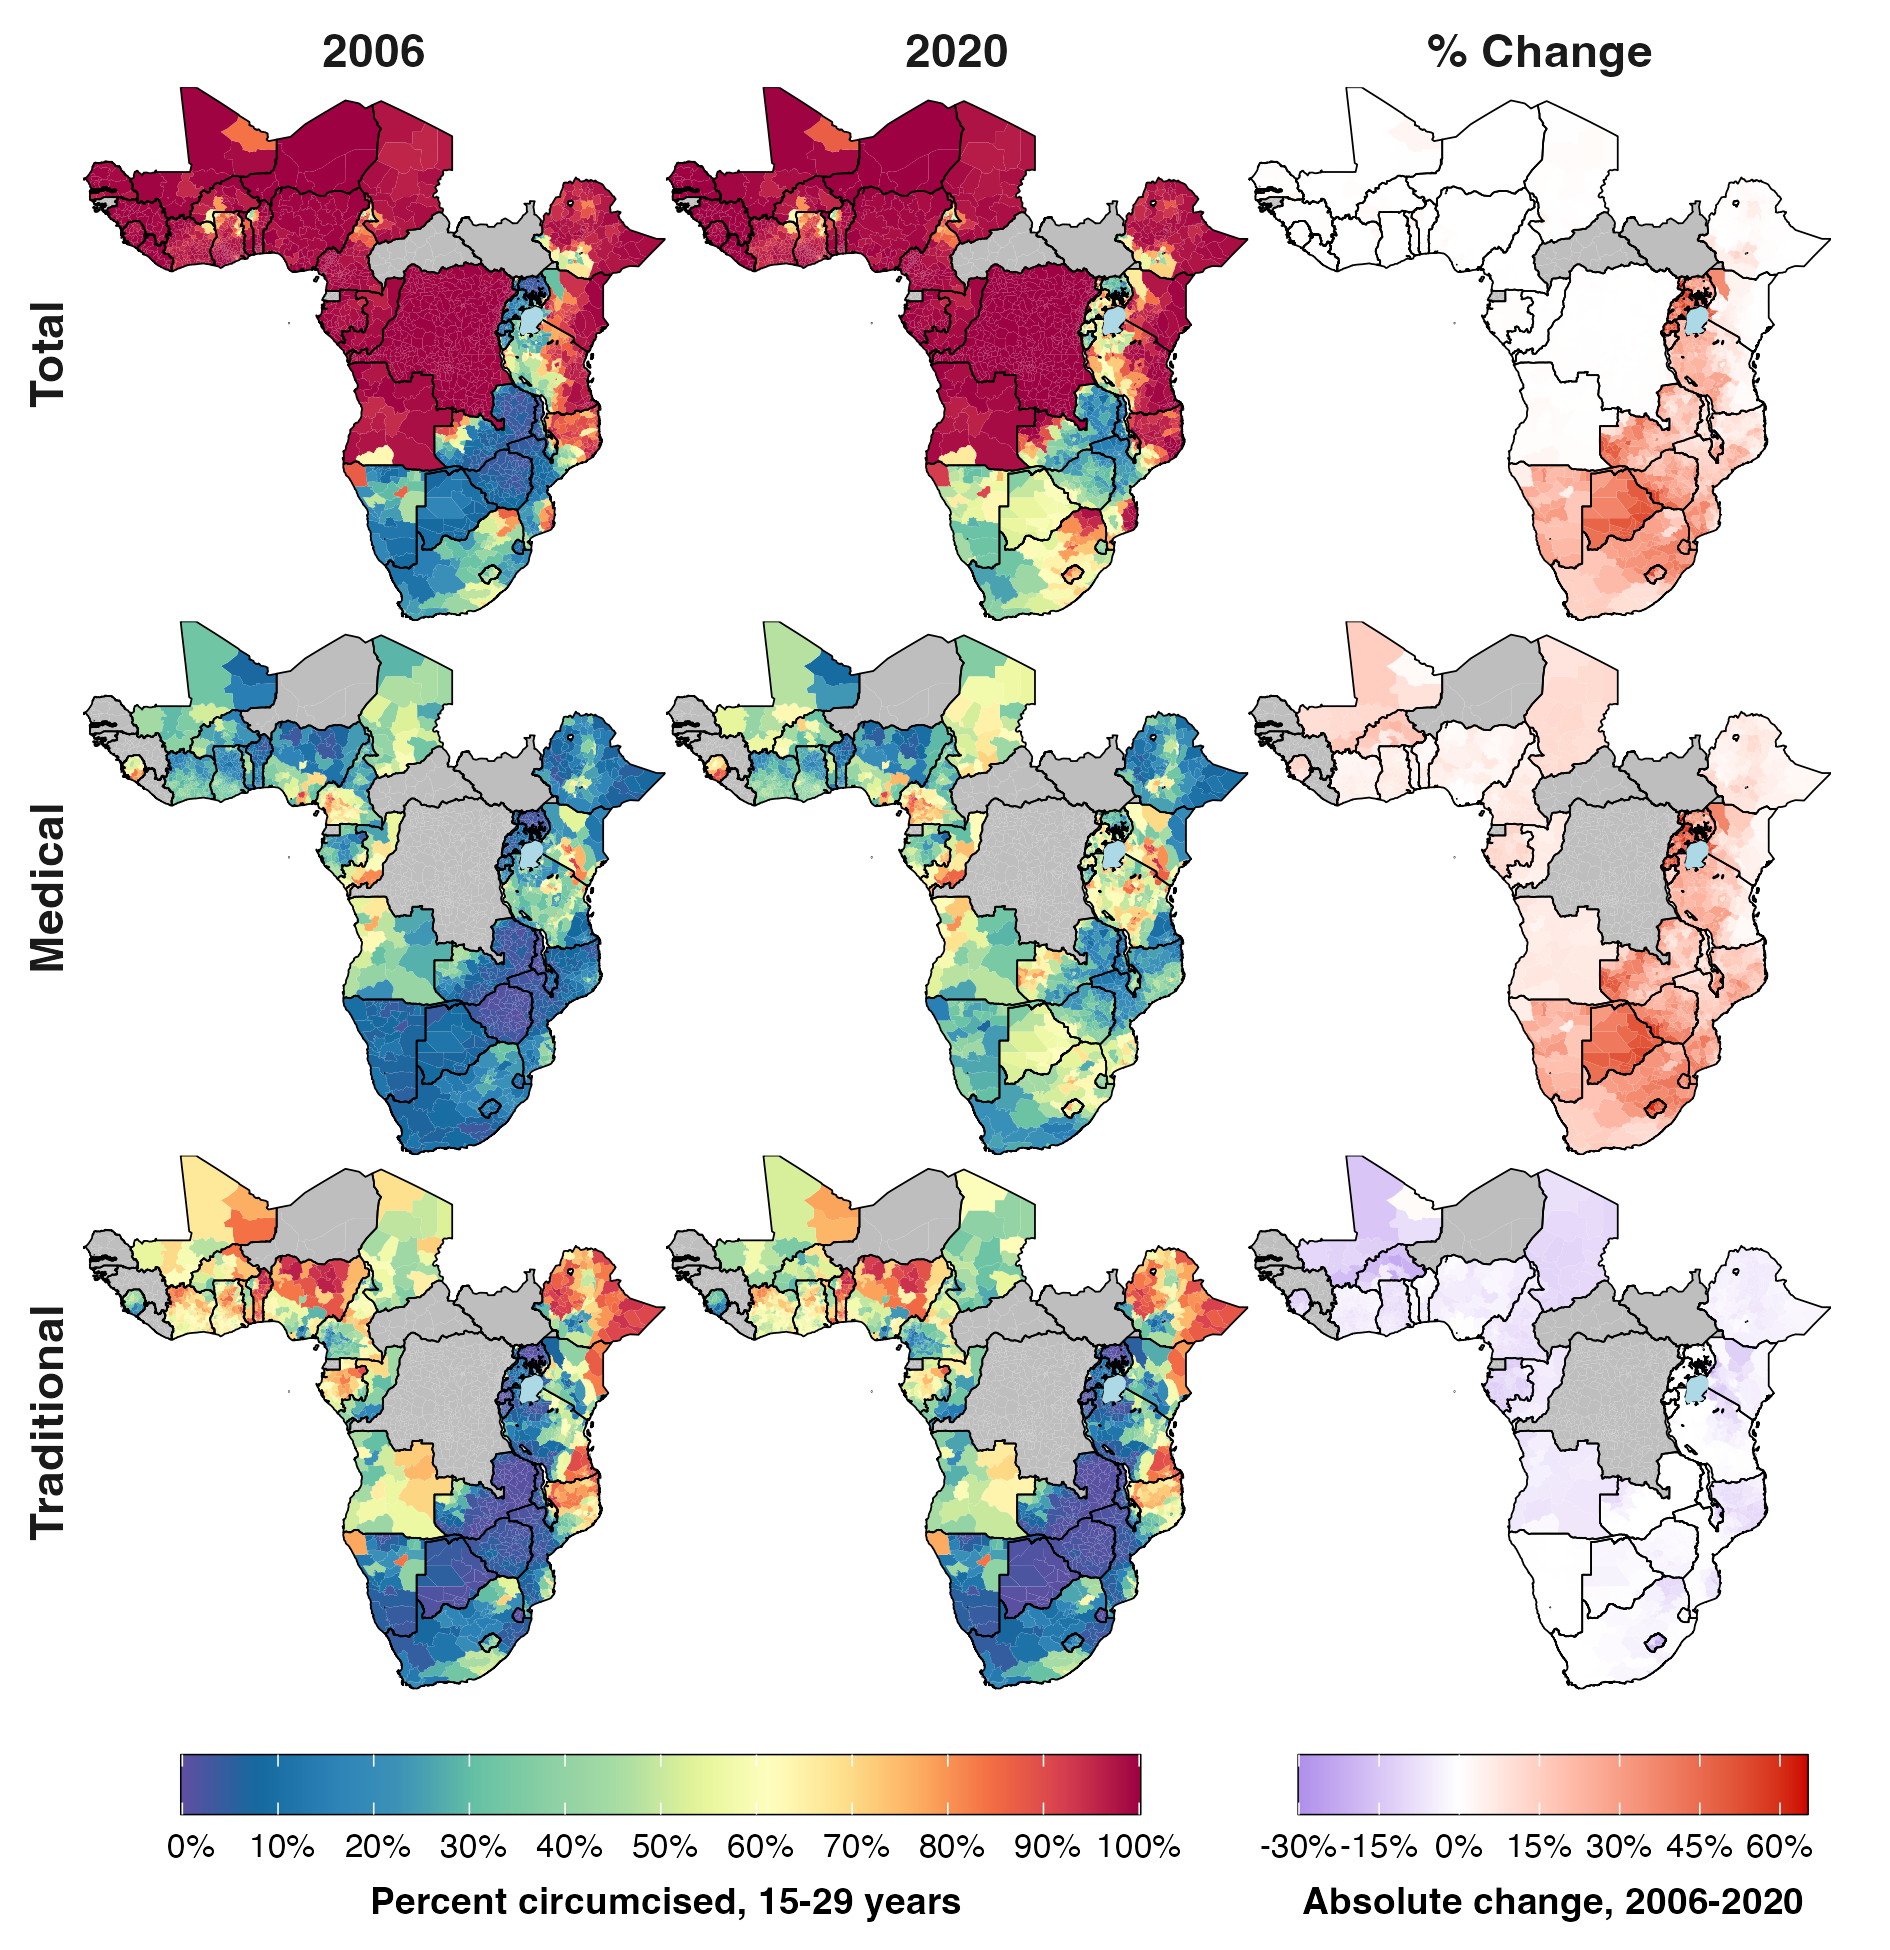
\includegraphics[width=1\linewidth]
    {figures/paper/01_map_plot_facet.png}
    \caption{\emph{Estimated percentage of men aged 15-29 years who were circumcised sub-nationally in 33 sub-Saharan African countries in 2006 and 2020, as well as the difference in coverage between the two years. Maps show total male circumcision (MC), medical male circumcision (MMC) and traditional male circumcision (TMC), respectively. Countries with no information on circumcision type are grey in the Medical and Traditional figures/paper, while countries with no circumcision estimate are grey in all.}}
    \label{fig::coveragemap}
\end{figure}

\begin{figure}[H]
    \centering
    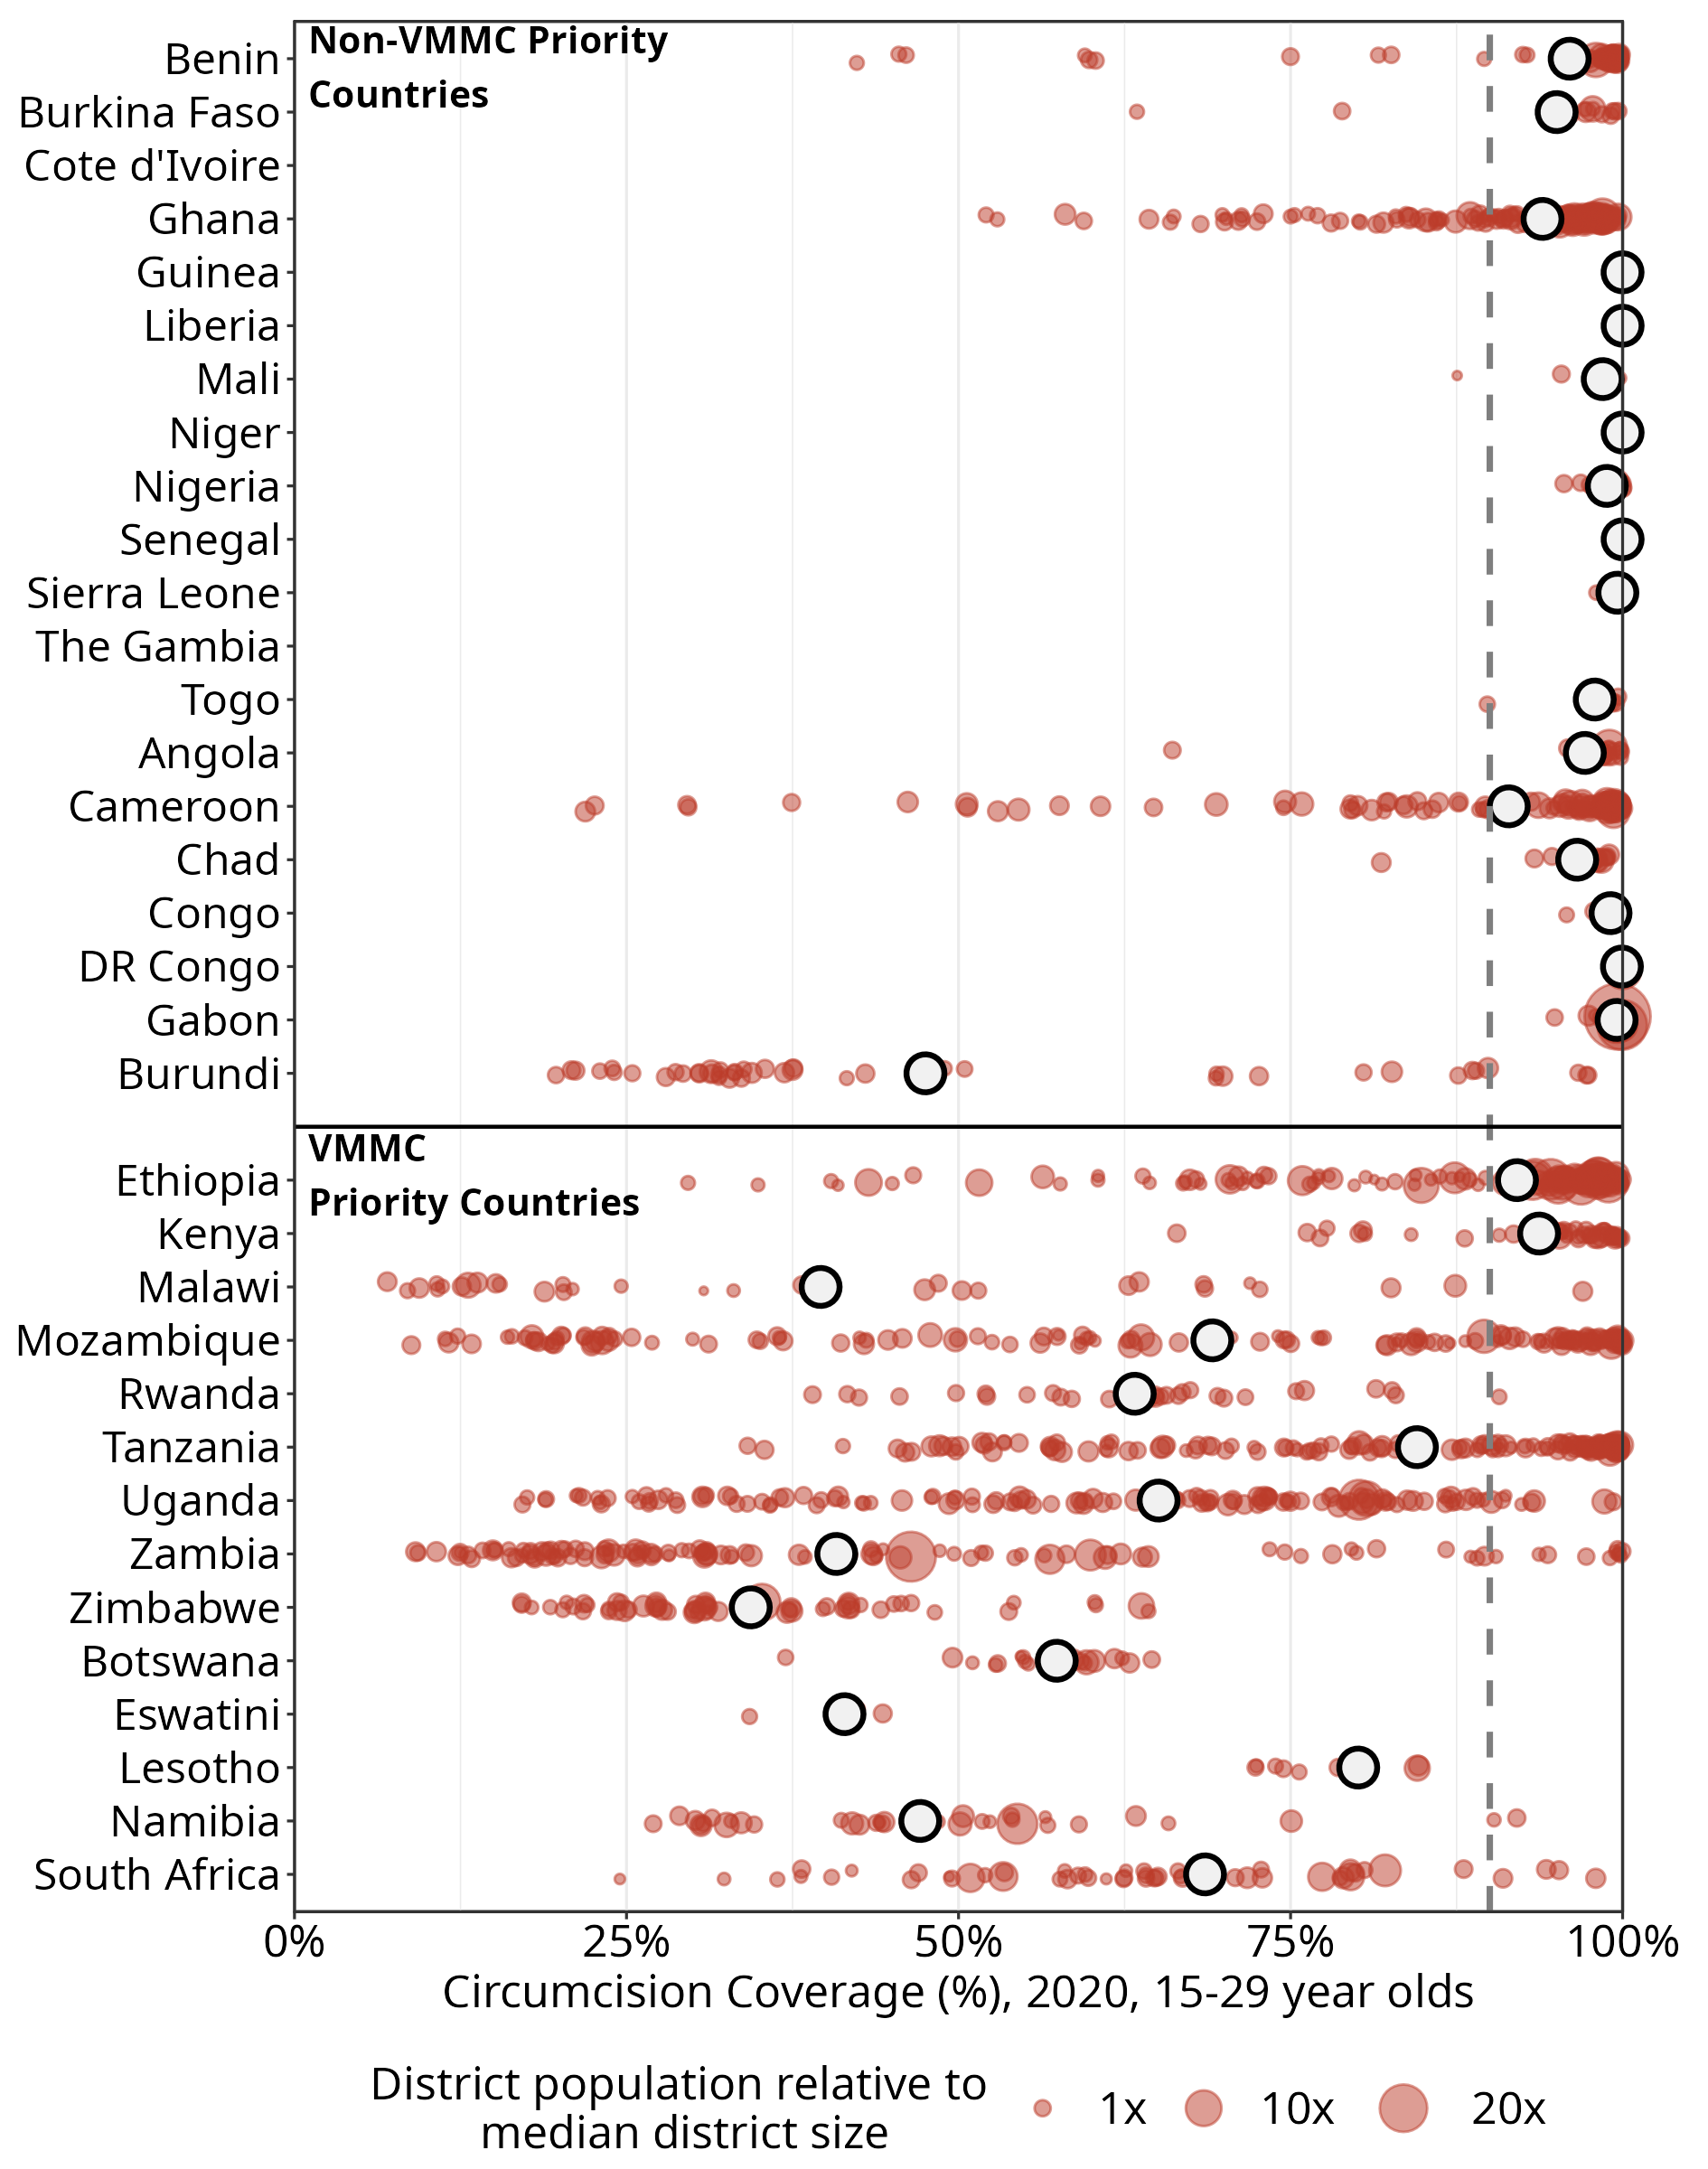
\includegraphics[width=.9\linewidth]
    {figures/paper/02_subnat_plot.png}
    \caption{\emph{District-level median percentage of men aged 15-29 years who were circumcised in 2020 in 33 SSA countries.
    Each point is a district, sized by district population relative to average district size.
    Each white dot represents the national median. 
    A vertical dotted line signifies the UNAIDS target of 90\% national male circumcision amongst 15-29 year olds. The countries below the horizontal black line are VMMC priority countries. VMMC = Voluntary Medical Male Circumcision.}}
    \label{fig::coveragedotplot}
\end{figure}

\begin{figure}[H]
    \centering
    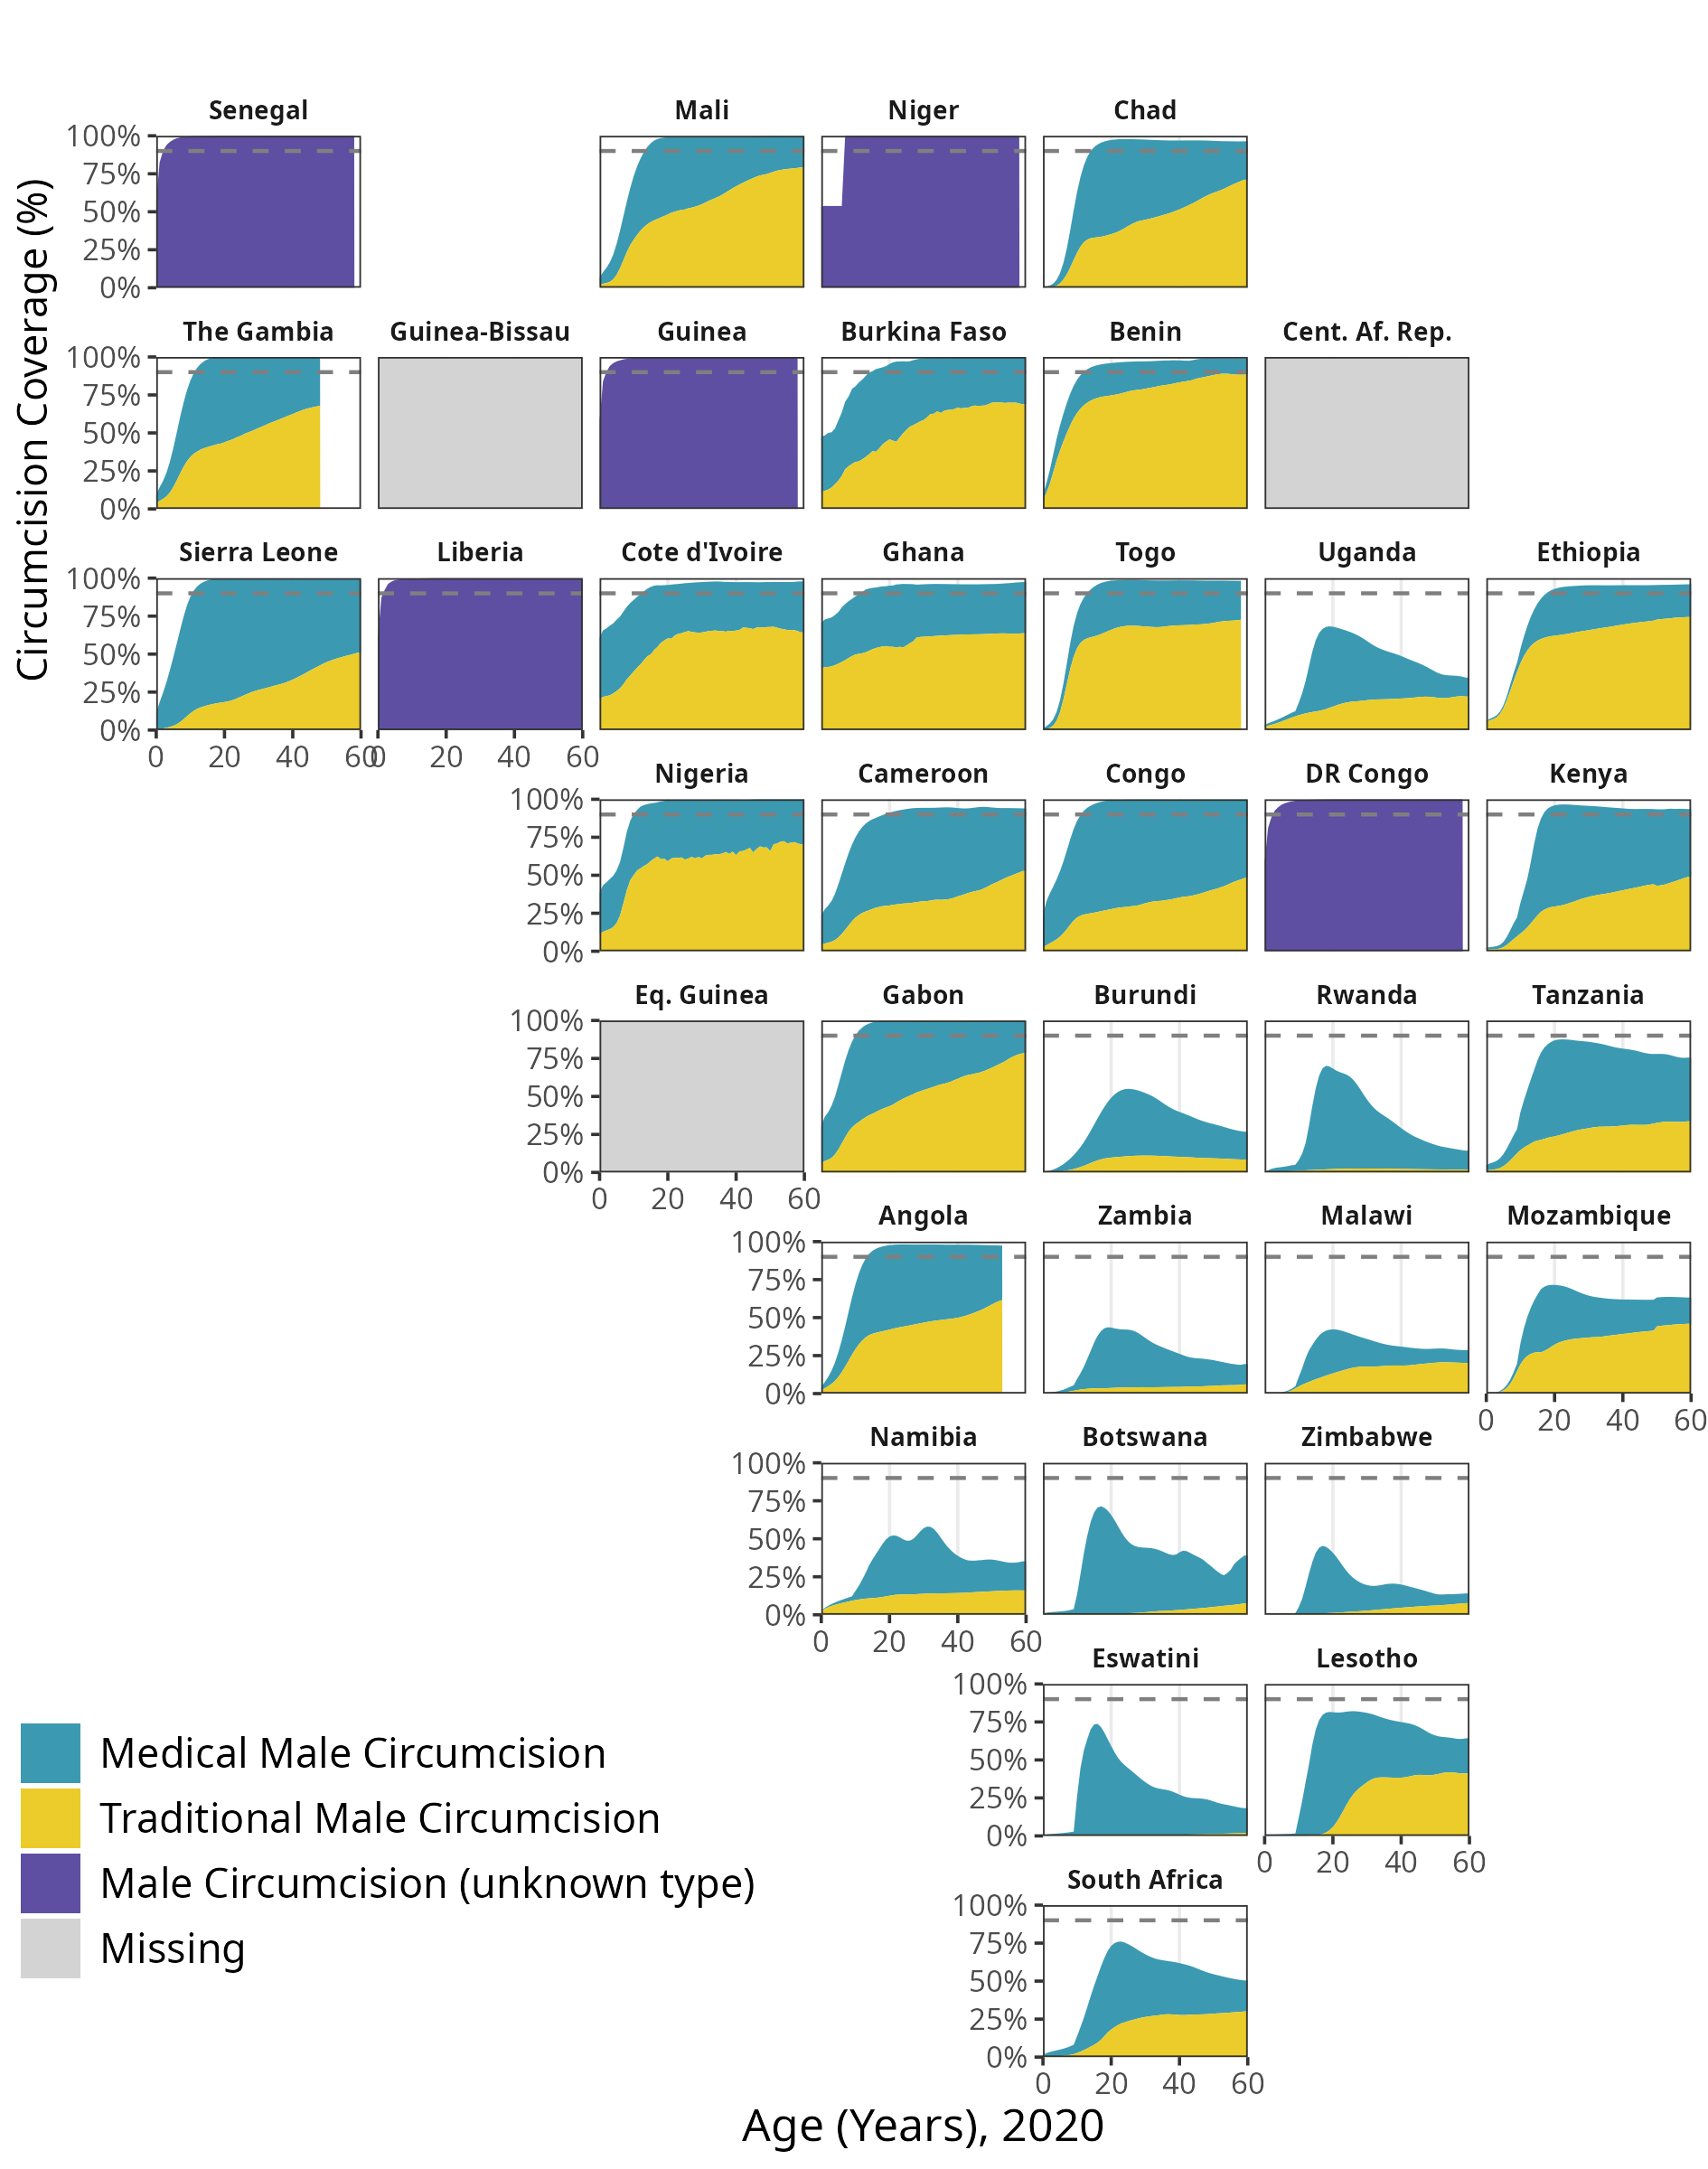
\includegraphics[width=.9\linewidth]
    {figures/paper/03_geo_age.png}
    \caption{\emph{Projected percentage of men from 0 to 60 years old who were medically circumcised and traditionally circumcised by 2020. The horizontal grey dashed line indicates the 90\% circumcision coverage by 2021 target established by the UNAIDS Fast Track strategy. Purple areas represent countries where circumcision type could not be ascertained from surveys, and so shows total male circumcision. Cent. Af. Rep. = Central African Republic, Eq. Guinea = Equatorial Guinea.}}
\end{figure}

\begin{figure}[H]
    \centering
    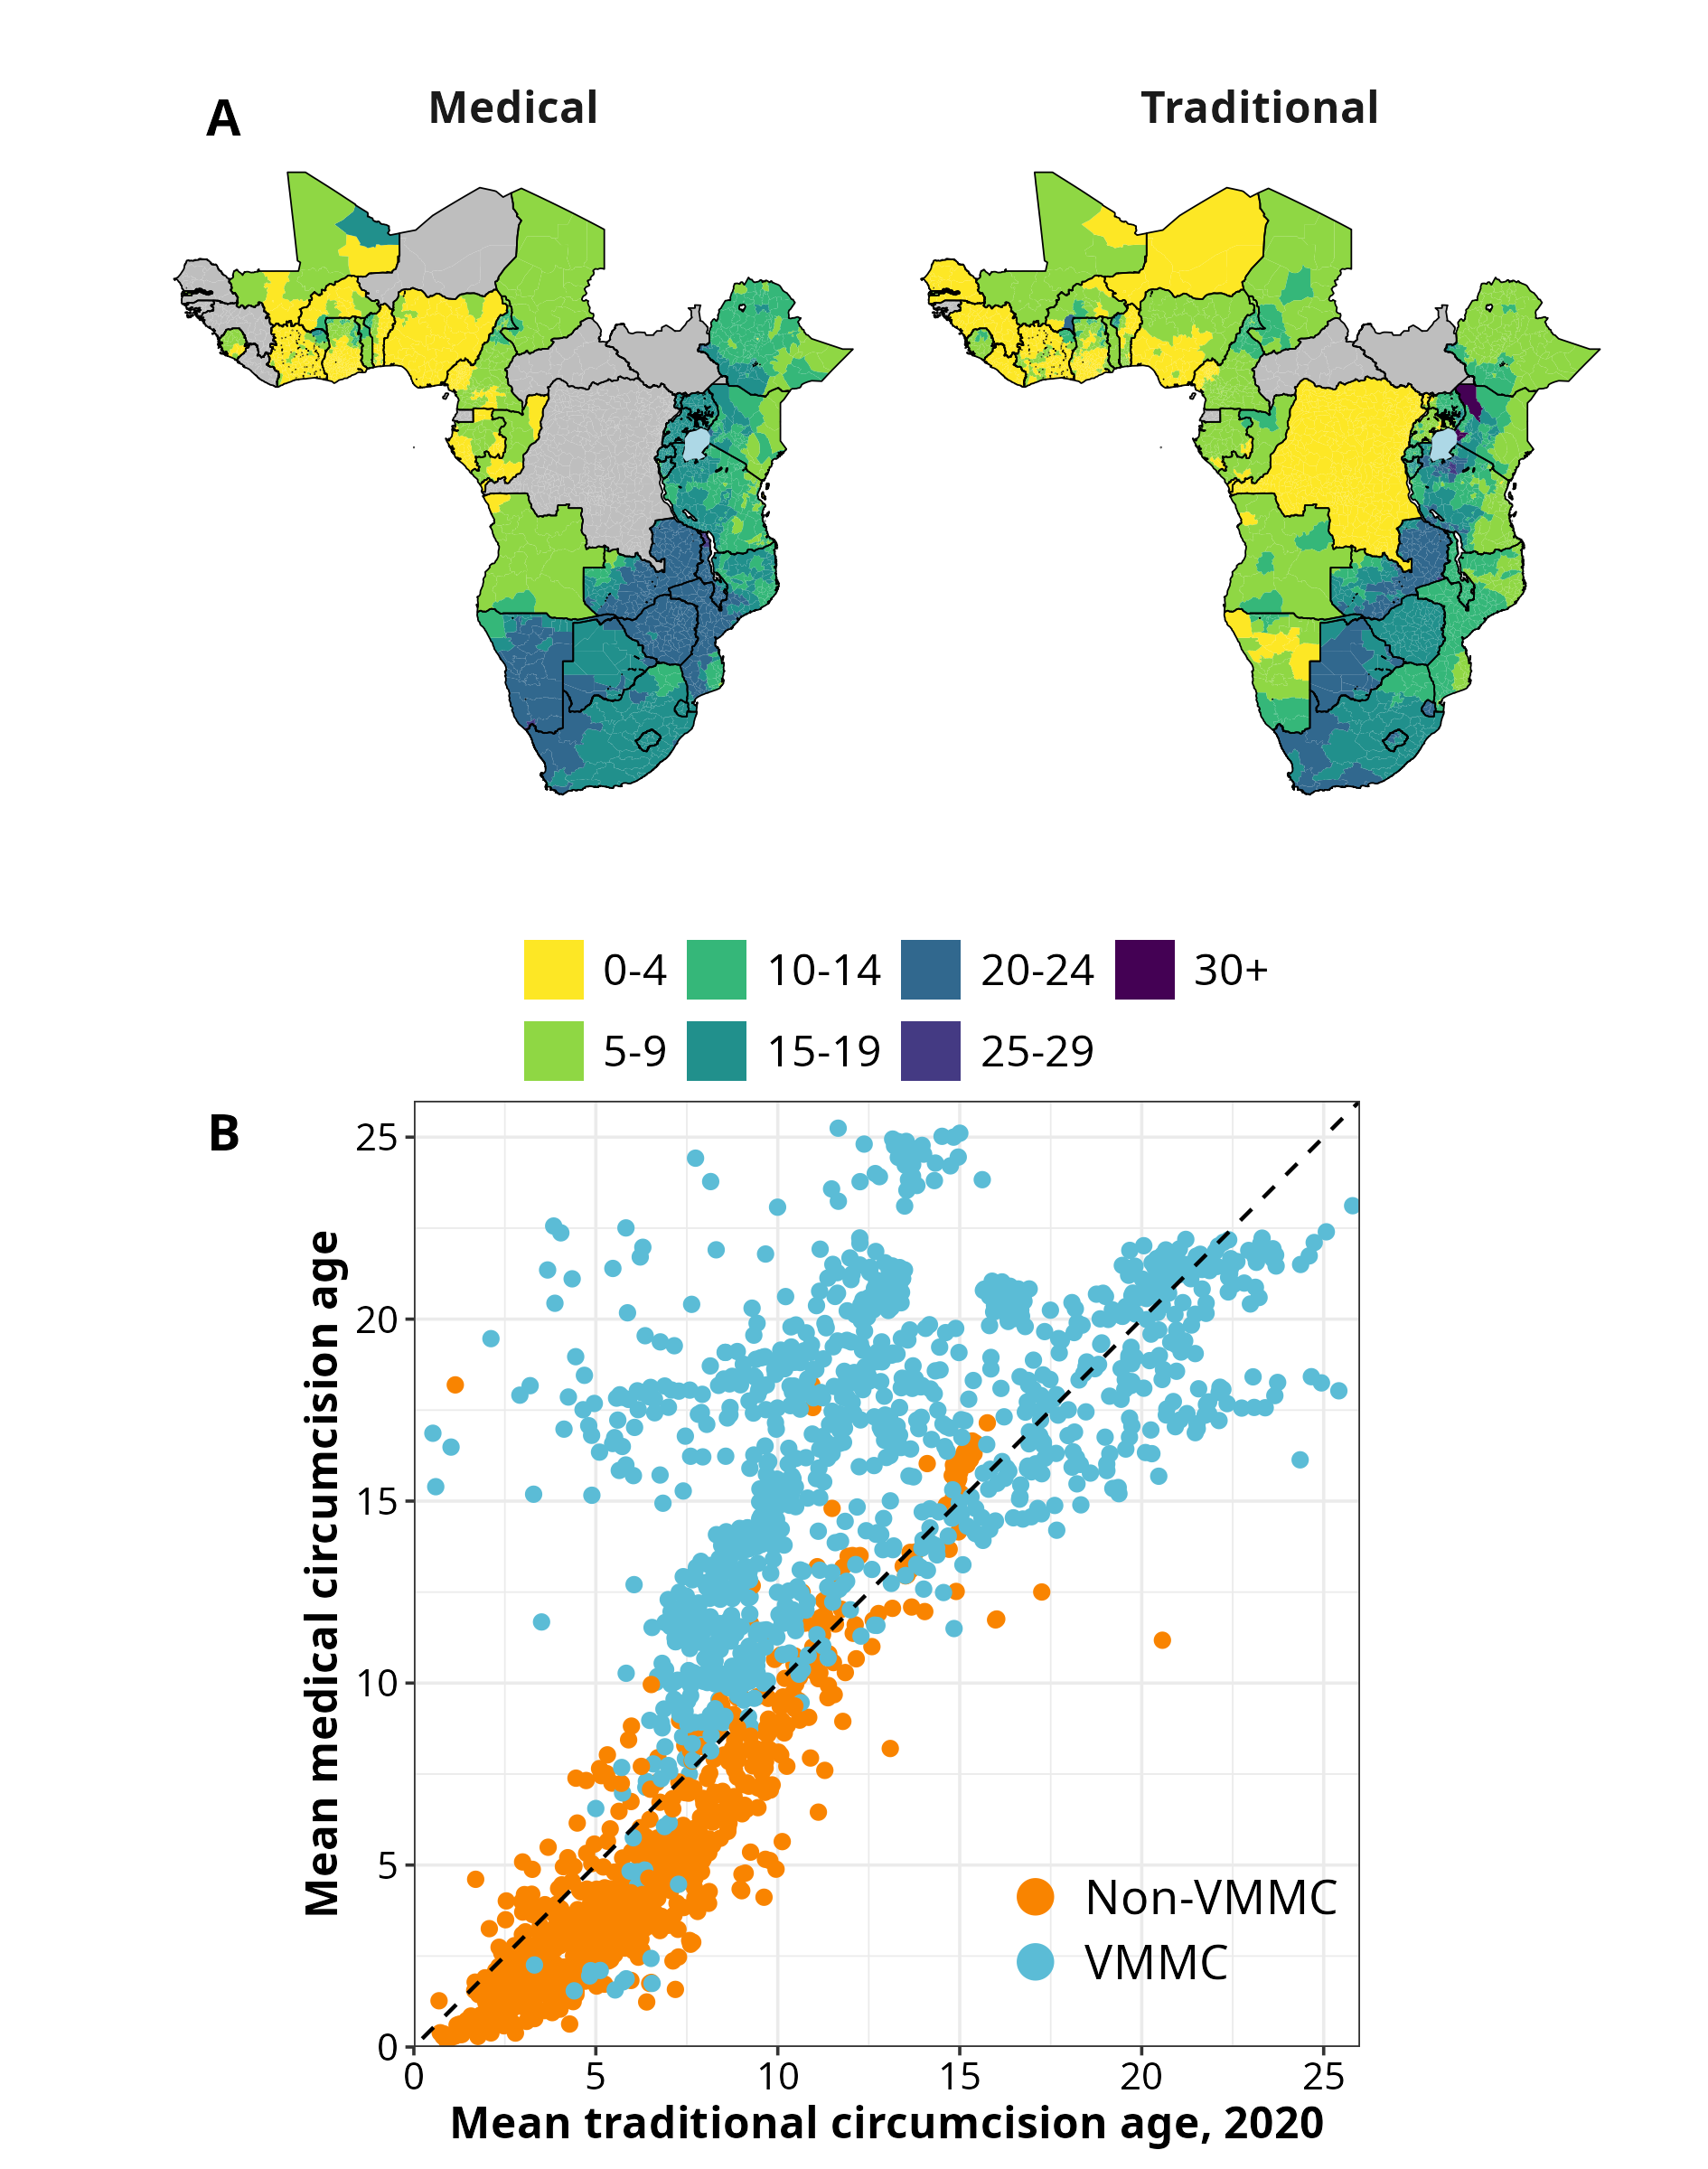
\includegraphics[width=.9\linewidth]
    {figures/paper/04_map_plot_mean_circ_age.png}
    \caption{\emph{(A) Estimated distinct-level age at circumcision in 2020 in 33 sub-Saharan African countries. Maps show mean medical male circumcision (MMC) and mean traditional male circumcision (TMC) age. Countries without estimates are in grey. Countries with no information on circumcision type have male circumcision (MC) displayed in the TMC plot, and are coloured in grey in the MMC plot. Mean circumcision ages are binned into five-year age groups and over 30s. (B) Scatterplot of district-level mean traditional male circumcision age versus mean medical male circumcision age. A diagonal dashed line passes through the origin and (25, 25). Points representing each district are coloured by whether their country is a Voluntary Male Medical Circumcision (VMMC) priority country.}}
\end{figure}

\begin{figure}[H]
    \centering
    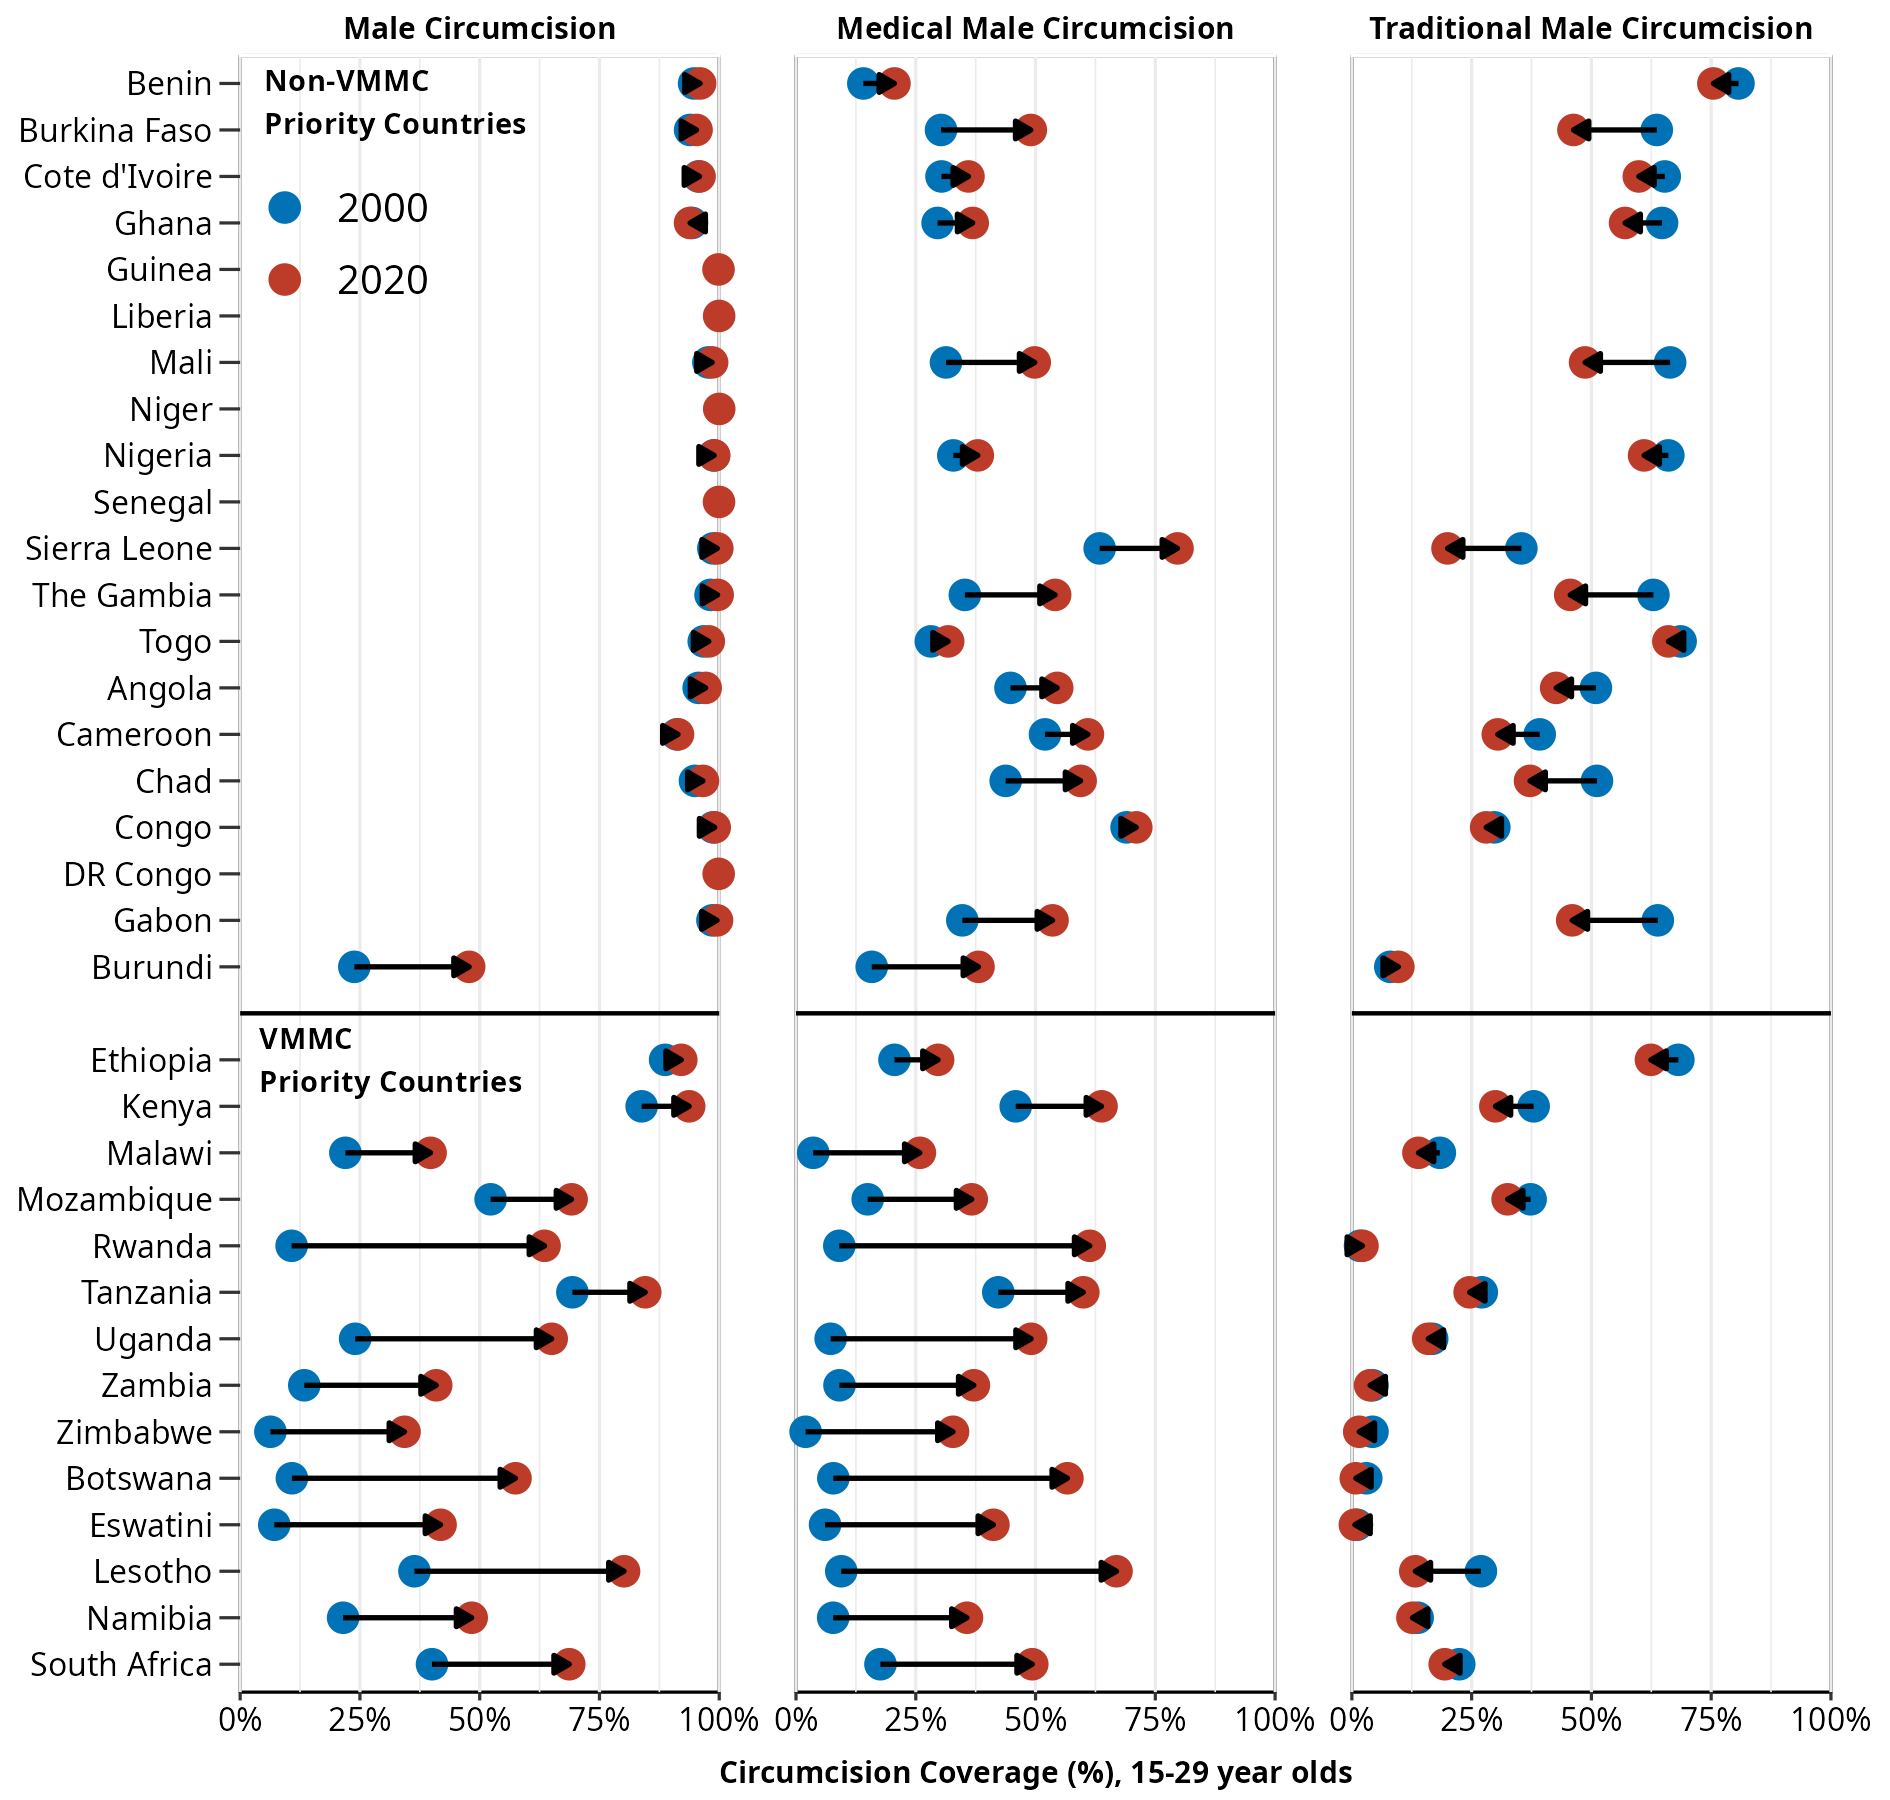
\includegraphics[width=1\linewidth]
    {figures/paper/05_change_00_20.png}
    % \caption{\emph{Absolute difference, in percentage coverage from 2000 to 2020, coloured by sub-Saharan African region. figures/paper are split by circumcision type. Countries are ordered from north to south, east to west, and the 13 countries below the black horizontal lines are VMMC priority countries.  }}
    \caption{\emph{Circumcision coverage in 2000 and 2020 amongst 15-29 year olds in all 34 sub-Saharan African countries, split by circumcision type. The countries below the horizontal black line are VMMC priority countries.}}
\end{figure}



%%%%%%%%%%%%%%%%%%%%%%%%%%%%%%%%%%%%%%%%%%%%%%%%%%%%%%%%%%%%%%%%%%
%%%%%%%%%%%%%%%%%%%%%%%%%%%%%%%%%%%%%%%%%%%%%%%%%%%%%%%%%%%%%%%%%%
%%%%%%%%%%%%%%%%%%%%%%%%%%%%%%%%%%%%%%%%%%%%%%%%%%%%%%%%%%%%%%%%%%

\end{document}

%%%%%%%%%%%%%%%%%%%%%%%%%%%%%%%%%%%%%%%%%%%%%%%%%%%%%%%%%%%%%%%%%%
%%%%%%%%%%%%%%%%%%%%%%%%%%%%%%%%%%%%%%%%%%%%%%%%%%%%%%%%%%%%%%%%%%
%%%%%%%%%%%%%%%%%%%%%%%%%%%%%%%%%%%%%%%%%%%%%%%%%%%%%%%%%%%%%%%%%%